%==============================================================================
% tento soubor pouzijte jako zaklad
% this file should be used as a base for the thesis
% Autoři / Authors: 2008 Michal Bidlo, 2019 Jaroslav Dytrych
% Kontakt pro dotazy a připomínky: sablona@fit.vutbr.cz
% Contact for questions and comments: sablona@fit.vutbr.cz
%==============================================================================
% kodovani: UTF-8 (zmena prikazem iconv, recode nebo cstocs)
% encoding: UTF-8 (you can change it by command iconv, recode or cstocs)
%------------------------------------------------------------------------------
% zpracování / processing: make, make pdf, make clean
%==============================================================================
% Soubory, které je nutné upravit nebo smazat: / Files which have to be edited or deleted:
%   projekt-20-literatura-bibliography.bib - literatura / bibliography
%   projekt-01-kapitoly-chapters.tex - obsah práce / the thesis content
%   projekt-01-kapitoly-chapters-en.tex - obsah práce v angličtině / the thesis content in English
%   projekt-30-prilohy-appendices.tex - přílohy / appendices
%   projekt-30-prilohy-appendices-en.tex - přílohy v angličtině / appendices in English
%==============================================================================
\documentclass[]{fitthesis} % bez zadání - pro začátek práce, aby nebyl problém s překladem
%\documentclass[english]{fitthesis} % without assignment - for the work start to avoid compilation problem
%\documentclass[zadani]{fitthesis} % odevzdani do wisu a/nebo tisk s barevnými odkazy - odkazy jsou barevné
%\documentclass[english,zadani]{fitthesis} % for submission to the IS FIT and/or print with color links - links are color
%\documentclass[zadani,print]{fitthesis} % pro černobílý tisk - odkazy jsou černé
%\documentclass[english,zadani,print]{fitthesis} % for the black and white print - links are black
%\documentclass[zadani,cprint]{fitthesis} % pro barevný tisk - odkazy jsou černé, znak VUT barevný
%\documentclass[english,zadani,cprint]{fitthesis} % for the print - links are black, logo is color
% * Je-li práce psaná v anglickém jazyce, je zapotřebí u třídy použít 
%   parametr english následovně:
%   If thesis is written in English, it is necessary to use 
%   parameter english as follows:
%      \documentclass[english]{fitthesis}
% * Je-li práce psaná ve slovenském jazyce, je zapotřebí u třídy použít 
%   parametr slovak následovně:
%   If the work is written in the Slovak language, it is necessary 
%   to use parameter slovak as follows:
%      \documentclass[slovak]{fitthesis}
% * Je-li práce psaná v anglickém jazyce se slovenským abstraktem apod., 
%   je zapotřebí u třídy použít parametry english a enslovak následovně:
%   If the work is written in English with the Slovak abstract, etc., 
%   it is necessary to use parameters english and enslovak as follows:
%      \documentclass[english,enslovak]{fitthesis}

% Základní balíčky jsou dole v souboru šablony fitthesis.cls
% Basic packages are at the bottom of template file fitthesis.cls
% zde můžeme vložit vlastní balíčky / you can place own packages here

% Kompilace po částech (rychlejší, ale v náhledu nemusí být vše aktuální)
% Compilation piecewise (faster, but not all parts in preview will be up-to-date)
% \usepackage{subfiles}

% Nastavení cesty k obrázkům
% Setting of a path to the pictures
%\graphicspath{{obrazky-figures/}{./obrazky-figures/}}
%\graphicspath{{obrazky-figures/}{../obrazky-figures/}}

%---rm---------------
\renewcommand{\rmdefault}{lmr}%zavede Latin Modern Roman jako rm / set Latin Modern Roman as rm
%---sf---------------
\renewcommand{\sfdefault}{qhv}%zavede TeX Gyre Heros jako sf
%---tt------------
\renewcommand{\ttdefault}{lmtt}% zavede Latin Modern tt jako tt

% vypne funkci šablony, která automaticky nahrazuje uvozovky,
% aby nebyly prováděny nevhodné náhrady v popisech API apod.
% disables function of the template which replaces quotation marks
% to avoid unnecessary replacements in the API descriptions etc.
\csdoublequotesoff



\usepackage{url}


% =======================================================================
% balíček "hyperref" vytváří klikací odkazy v pdf, pokud tedy použijeme pdflatex
% problém je, že balíček hyperref musí být uveden jako poslední, takže nemůže
% být v šabloně
% "hyperref" package create clickable links in pdf if you are using pdflatex.
% Problem is that this package have to be introduced as the last one so it 
% can not be placed in the template file.
\ifWis
\ifx\pdfoutput\undefined % nejedeme pod pdflatexem / we are not using pdflatex
\else
  \usepackage{color}
  \usepackage[unicode,colorlinks,hyperindex,plainpages=false,pdftex]{hyperref}
  \definecolor{hrcolor-ref}{RGB}{223,52,30}
  \definecolor{hrcolor-cite}{HTML}{2F8F00}
  \definecolor{hrcolor-urls}{HTML}{092EAB}
  \hypersetup{
	linkcolor=hrcolor-ref,
	citecolor=hrcolor-cite,
	filecolor=magenta,
	urlcolor=hrcolor-urls
  }
  \def\pdfBorderAttrs{/Border [0 0 0] }  % bez okrajů kolem odkazů / without margins around links
  \pdfcompresslevel=9
\fi
\else % pro tisk budou odkazy, na které se dá klikat, černé / for the print clickable links will be black
\ifx\pdfoutput\undefined % nejedeme pod pdflatexem / we are not using pdflatex
\else
  \usepackage{color}
  \usepackage[unicode,colorlinks,hyperindex,plainpages=false,pdftex,urlcolor=black,linkcolor=black,citecolor=black]{hyperref}
  \definecolor{links}{rgb}{0,0,0}
  \definecolor{anchors}{rgb}{0,0,0}
  \def\AnchorColor{anchors}
  \def\LinkColor{links}
  \def\pdfBorderAttrs{/Border [0 0 0] } % bez okrajů kolem odkazů / without margins around links
  \pdfcompresslevel=9
\fi
\fi
% Řešení problému, kdy klikací odkazy na obrázky vedou za obrázek
% This solves the problems with links which leads after the picture
\usepackage[all]{hypcap}

% Informace o práci/projektu / Information about the thesis
%---------------------------------------------------------------------------
\projectinfo{
  %Prace / Thesis
  project={BP},            %typ práce BP/SP/DP/DR  / thesis type (SP = term project)
  year={2020},             % rok odevzdání / year of submission
  date=\today,             % datum odevzdání / submission date
  %Nazev prace / thesis title
  title.cs={Generování sekvenčních diagramů z modelů Petriho sítí},  % název práce v češtině či slovenštině (dle zadání) / thesis title in czech language (according to assignment)
  title.en={Generating sequence diagrams based on petri nets}, % název práce v angličtině / thesis title in english
  %title.length={14.5cm}, % nastavení délky bloku s titulkem pro úpravu zalomení řádku (lze definovat zde nebo níže) / setting the length of a block with a thesis title for adjusting a line break (can be defined here or below)
  %sectitle.length={14.5cm}, % nastavení délky bloku s druhým titulkem pro úpravu zalomení řádku (lze definovat zde nebo níže) / setting the length of a block with a second thesis title for adjusting a line break (can be defined here or below)
  %Autor / Author
  author.name={Erik},   % jméno autora / author name
  author.surname={Kelemen},   % příjmení autora / author surname 
  %author.title.p={Bc.}, % titul před jménem (nepovinné) / title before the name (optional)
  %author.title.a={Ph.D.}, % titul za jménem (nepovinné) / title after the name (optional)
  %Ustav / Department
  department={UPGM}, % doplňte příslušnou zkratku dle ústavu na zadání: UPSY/UIFS/UITS/UPGM / fill in appropriate abbreviation of the department according to assignment: UPSY/UIFS/UITS/UPGM
  % Školitel / supervisor
  supervisor.name={Radek},   % jméno školitele / supervisor name 
  supervisor.surname={Kočí},   % příjmení školitele / supervisor surname
  supervisor.title.p={Ing.},   %titul před jménem (nepovinné) / title before the name (optional)
  supervisor.title.a={Ph.D.},    %titul za jménem (nepovinné) / title after the name (optional)
  % Klíčová slova / keywords
  keywords.cs={objektovo orientované petriho siete, sekvenčný diagram, simulácia.}, % klíčová slova v českém či slovenském jazyce / keywords in czech or slovak language
  keywords.en={object oriented petri nets, sequence diagram, simulation}, % klíčová slova v anglickém jazyce / keywords in english
  %keywords.en={Here, individual keywords separated by commas will be written in English.},
  % Abstrakt / Abstract
  abstract.cs={Zatiaľ čo petriho siete nesporne dominujú v monitorovaní zmeny stavov v modelovanom systéme, sekvenčné diagramy dokážu lepšie prezentovať externý pohľad na systém v časovom slede posielaných správ. Hlavným cieľom tejto bakalárskej práce je vygenerovať sekvenčný diagram pomocou simulácie modelu objektovo orientovanej petriho siete zapísaného v jazyku PNTalk. Práca sa zaoberá transformáciou dát v zmysle minimálnej straty informácie z modelu objektovo orientovaných peteriho sietí a následnú prezentáciu vyťažených dát nad rámec triviálnych sekvenčných diagramov. }, % abstrakt v českém či slovenském jazyce / abstract in czech or slovak language
  abstract.en={Do tohoto odstavce bude zapsán výtah (abstrakt) práce v anglickém jazyce.}, % abstrakt v anglickém jazyce / abstract in english
  %abstract.en={An abstract of the work in English will be written in this paragraph.},
  % Prohlášení (u anglicky psané práce anglicky, u slovensky psané práce slovensky) / Declaration (for thesis in english should be in english)
  declaration={Prohlašuji, že jsem tuto bakalářskou práci vypracoval samostatně pod vedením pana Radek Kočí.
Další informace mi poskytli Tomáš Lapšanský ako konzultant práce na ktorú som priamo nadviazal.
Uvedl jsem všechny literární prameny, publikace a další zdroje, ze kterých jsem čerpal.},
  %declaration={I hereby declare that this Bachelor's thesis was prepared as an original work by the author under the supervision of Mr. X
% The supplementary information was provided by Mr. Y
% I have listed all the literary sources, publications and other sources, which were used during the preparation of this thesis.},
  % Poděkování (nepovinné, nejlépe v jazyce práce) / Acknowledgement (optional, ideally in the language of the thesis)
  acknowledgment={V této sekci je možno uvést poděkování vedoucímu práce a těm, kteří poskytli odbornou pomoc
(externí zadavatel, konzultant apod.).},
  %acknowledgment={Here it is possible to express thanks to the supervisor and to the people which provided professional help
%(external submitter, consultant, etc.).},
  % Rozšířený abstrakt (cca 3 normostrany) - lze definovat zde nebo níže / Extended abstract (approximately 3 standard pages) - can be defined here or below
  %extendedabstract={Do tohoto odstavce bude zapsán rozšířený výtah (abstrakt) práce v českém (slovenském) jazyce.},
  %faculty={FIT}, % FIT/FEKT/FSI/FA/FCH/FP/FAST/FAVU/USI/DEF
  faculty.cs={Fakulta informačních technologií}, % Fakulta v češtině - pro využití této položky výše zvolte fakultu DEF / Faculty in Czech - for use of this entry select DEF above
  faculty.en={Faculty of Information Technology}, % Fakulta v angličtině - pro využití této položky výše zvolte fakultu DEF / Faculty in English - for use of this entry select DEF above
  department.cs={Ústav matematiky}, % Ústav v češtině - pro využití této položky výše zvolte ústav DEF nebo jej zakomentujte / Department in Czech - for use of this entry select DEF above or comment it out
  department.en={Institute of Mathematics} % Ústav v angličtině - pro využití této položky výše zvolte ústav DEF nebo jej zakomentujte / Department in English - for use of this entry select DEF above or comment it out
}

% Rozšířený abstrakt (cca 3 normostrany) - lze definovat zde nebo výše / Extended abstract (approximately 3 standard pages) - can be defined here or above
%\extendedabstract{Do tohoto odstavce bude zapsán výtah (abstrakt) práce v českém (slovenském) jazyce.}

% nastavení délky bloku s titulkem pro úpravu zalomení řádku - lze definovat zde nebo výše / setting the length of a block with a thesis title for adjusting a line break - can be defined here or above
%\titlelength{14.5cm}
% nastavení délky bloku s druhým titulkem pro úpravu zalomení řádku - lze definovat zde nebo výše / setting the length of a block with a second thesis title for adjusting a line break - can be defined here or above
%\sectitlelength{14.5cm}

% řeší první/poslední řádek odstavce na předchozí/následující stránce
% solves first/last row of the paragraph on the previous/next page
\clubpenalty=10000
\widowpenalty=10000

% checklist
\newlist{checklist}{itemize}{1}
\setlist[checklist]{label=$\square$}

\begin{document}
  % Vysazeni titulnich stran / Typesetting of the title pages
  % ----------------------------------------------
  \maketitle
  % Obsah
  % ----------------------------------------------
  \setlength{\parskip}{0pt}

  {\hypersetup{hidelinks}\tableofcontents}
  
  % Seznam obrazku a tabulek (pokud prace obsahuje velke mnozstvi obrazku, tak se to hodi)
  % List of figures and list of tables (if the thesis contains a lot of pictures, it is good)
  \ifczech
    \renewcommand\listfigurename{Seznam obrázků}
  \fi
  \ifslovak
    \renewcommand\listfigurename{Zoznam obrázkov}
  \fi
  % {\hypersetup{hidelinks}\listoffigures}
  
  \ifczech
    \renewcommand\listtablename{Seznam tabulek}
  \fi
  \ifslovak
    \renewcommand\listtablename{Zoznam tabuliek}
  \fi
  % {\hypersetup{hidelinks}\listoftables}

  \ifODSAZ
    \setlength{\parskip}{0.5\bigskipamount}
  \else
    \setlength{\parskip}{0pt}
  \fi

  % vynechani stranky v oboustrannem rezimu
  % Skip the page in the two-sided mode
  \iftwoside
    \cleardoublepage
  \fi

  % Text prace / Thesis text
  % ----------------------------------------------
  \ifenglish
    \input{projekt-01-kapitoly-chapters-en}
  \else
    \theoremstyle{definition}
\newtheorem{defn}{Definícia}[section]
\newtheorem{note}{Poznámka}[section]
\newtheorem{exmpl}{Príklad}[section]

\chapter{Úvod}


Jeden z najzákladnejších problémov, ktoré rieši softvérový vývoj je validácia požiadavkov systému. Tieto požiadavky sú zvyčajne definované pomocou diagramu užitia z UML. 
Bežný postup je navrhnúť model systému podľa týchto požiadaviek za pomoci ostatných diagramov z UML a otestovať ho manuálne implementovaným prototypom. To predstavuje dosť práce jednak s diagramami UML a navyše implementovaný prototyp pravdepodobne stratí veškeré využitie po validácii modelu. Predstavme si však, že vytvoríme model za použitia objektovo orientovaných petriho sietí, ktorý prichádza s možnosťou simulácie modelu. Táto simulácia poskytuje priestor na automatické vytvorenie UML diagramov. Isteže existujú aj rozšírenia UML a metódy na ich prevod do spustiteľnej formy ako MDA methodology, Executable UML (xUML) language alebo Foundational Subset pre xUML, všetky zo zmienených metód však trpia nedostatkom, keď sa spustitelná forma UML modelu v priebehu validácie upravuje, je takmer nemožné vrátiť sa so zmenamy k pôvodnému modelu. 

Hlavným cieľom práce je vytvoriť plnohodnotný nástroj na validáciu modelu, ktorý vygeneruje sekvenčný diagram z jazyka UML. Jazyk UML definuje viac diagramov interakcií z ktorých by sa dalo vybrať, no narozdiel od diagramu interakcií sa dá vygenerovať zo simulácie a navyše je sekvenčný diagram druhý nanajvýš používaný z diagramov UML. Od nástroja sa očakáva, že by mal analyzovať všetky možné scenáre, rozlíšiť redundantné výskyty častí scenárov a agregovať ich, aby obmedzil zobrazované informácie. Ďalej by mal poskytovať intuitívne rozhranie a zachovať všetky informácie zo simulácie ľahko dohľadateľné.

Najzložitejšiu časť generovania sekvenčného diagramu predstavuje nahradzovanie dát potrebných na zostavenie sekvenčného diagramu, chýbajúcich v reprezentácii pomocou objektovo orientovaných petriho sietí.

V kapitole.. TODO

\chapter{Úvod2}

Jeden z najzákladnejších problémov, ktoré rieši softvérový vývoj v ranných fázach je modelovanie systému. K jednej zo zaužívaných variant pre modelovanie systému patrí jazyk UML (Unified Modeling Language) ku ktorému od roku 1997(štandart v1.1) patrí sekvenčný diagram ako jeden z diagramov na modelovanie interakcií v systéme. Na druhej strane máme Petriho siete(PT), matematický model, ktorý je schopný vyjadriť kauzalitu udalostí, asynchrónnost, paralelizmus a synchronizáciu. Petriho siete sa do UML dostali len ako inšpirácia pre diagram aktivít v roku 1999(v 1.3). Na prvý pohľad je zrejmé, že diagram interakcií s matematickým modelom Petriho sietí má pramálo spoločného a táto absencia relevantných informácii zrejme neumožňuje automatické generovanie z jedného modelu na druhý. 

To sa zmení pri transformácii PT Petriho sietí do  funkcionálnych Petriho sietí (FPN) a následnou transformáciou do objektovo orientovaných Petriho sietí (OOPN). Týmto prechodom sa priblížia invokačné prechody z funkcionálnych Petriho sietí k volaniam správ ako ich poznáme zo sekvenčných diagramov. Triedy OOPN sa priblížia k objektom sekvenčných diagramov. Táto analógia je základným stavebným kameňom pre vytvorenie funkčného generátoru sekvenčných diagramov z objektovo orientovaných Petriho sietí. Celá myšlienka pochádza z vedecko publicistického článku :TODO: reference 

Cieľom práce je okolo tejto myšlienky postaviť generátor, ktorého vstupom je kód jazyka PNTalk popisujúci OOPN a výstupom sekvenčný diagram. Na záver sa správnosť vygenerovaných diagramov posúdi v porovnaní s diagramami vytvorenými ručne odborníkami z praxe.

\chapter{Tvorba a analýza scenárov v modelovaní systému}

\section{Vývoj systému}

Pred ponorením sa do analýzy a modelovania softvéru, je nutno zmieniť, kde majú pri vývoji softvéru svoje miesto a aké aspekty ich ovplyvňujú.

\subsection{Zúčastnená strana}

Všetky fyzické osoby ovplyvňujúce vývoj softvéru môžme pre akýkoľvek systém klasifikovať do 5 skupín. Zobrazené sú na ľavej strane Obr. \ref{fig:system-inputs}. Podstatné je, že každá zo skupín má na systém iný uhol pohľadu.

\begin{enumerate}
	\item \textbf{Systémový analytici a projektový manažéri} sú špecialistami na analýzu a modelovanie, poskytujú ostatným skupinám poradenstvo a sú akýmsi mostom pri akomkoľvek komunikačnom šume vznikajúcom napríklad medzi menej technicky zdatnými majiteľmi a projektu a vývojármi.
	\item \textbf{Vývojári}, ktorý majú za úlohu celý systém zkonštruovať podľa návrhu softvérového dizajnéra riešia hlavne detaily implementácie. V menších firmách sú dizajnéry a vývojáry tí istí ľudia, no vo väčších sú tieto úlohy často oddelené.
	\item \textbf{Dizajnéri} zodpovedný za modelovanie architektúry systému z ich uhlu pohľadu riešia správnu voľbu technológie pre systém. Tendenciou je mať špecializovaného návrhára pre každú časť zvlášť, preto do tejto skupiny patria databázový administrátori, sieťový architekti, bezpečnostný experti a mnohí ďaľší.
	\item \textbf{Uživateľia} systému, sú v dnešnej dobe čím ďaľej technicky vyspelí a ďaľšou ich nespornou výhodou je počet, ktorý väčšinou prevyšuje ostatné skupiny. Z ich pohľadu na systém je najdôležitejšia funkcionalita, intuitívnosť používania a o cenu, či profit, narozdiel od majiteľov, nedbajú.
	\item \textbf{Majitelia} projektu, ktorých môže byť viac než jeden väčšinou riešia projekt z pohľadu financií. Na koľko ich to vyjde, aký bude profit, či benefity.
\end{enumerate}
\begin{figure}[H]
	\centering
	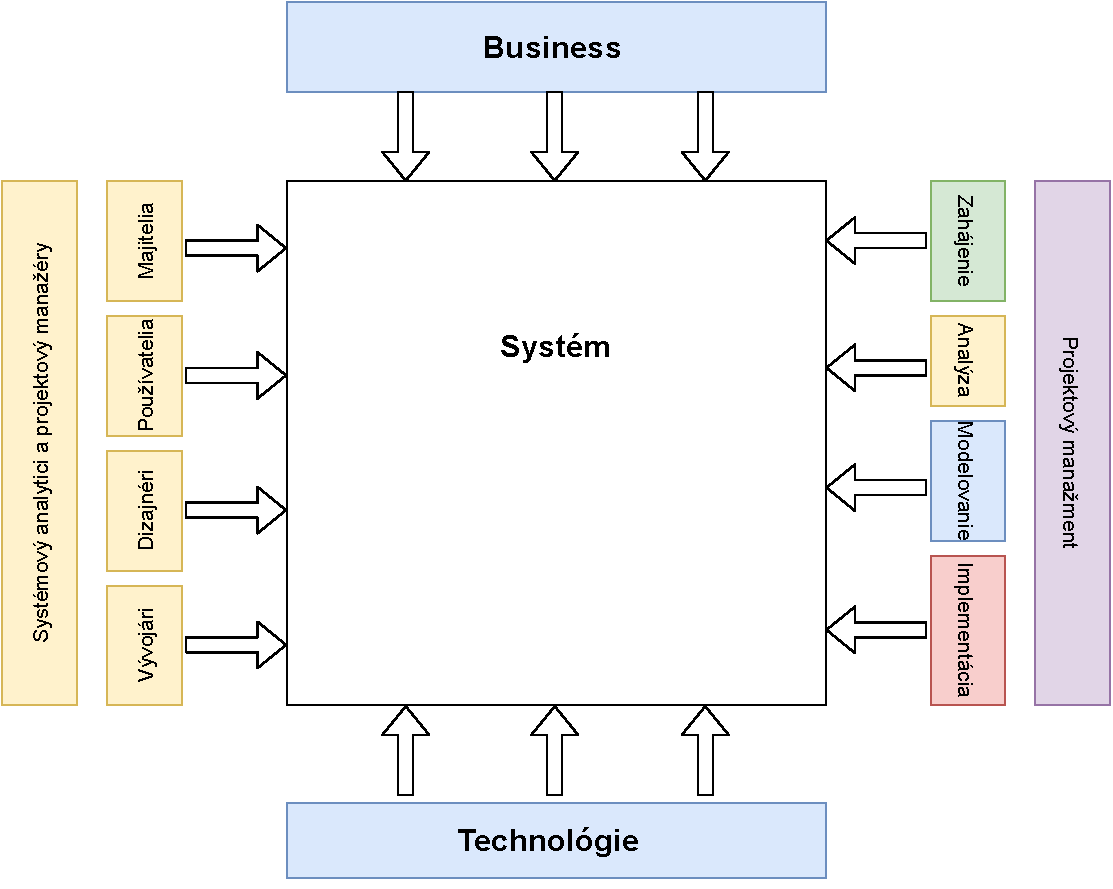
\includegraphics[scale=0.75]{obrazky-figures/TR-system-inputs}
	\caption{Aspekty ovplyvňujúce vývoj systému \cite{whitten2007systems}}
	\label{fig:system-inputs}
\end{figure}

\subsection{Iné factory}
Okrem Účastníkov vývoja majú na systém vplyv ešte aspekty businessu a technológie dostupné v dobe vývoja. Business pokrýva hlavne požiadavky obchodu spojené s legislatívou. Technológie nás obmedzujú pri nedostupnosti tak pokročilých technológií aké by sme potrebovali pre svoj systém alebo naopak nové prielomy v technológii poskytujú príležitosť pozdvihnnúť projekt na vyššiu úroveň.

\subsection{Procces vývoja}

Je zrejmé že väčšina organizácií bude mať vlastný formálne definovaný proces vývoja softvéru alebo sadu krokov, ktoré podľa ktorých by sa mal systém vyvíjať. Akiste sa budú tieto metodológie od seba diametrálne odlišovať pre jednotlivé organizácie. Avšak, všetky metódy riešenia problému môžeme zavšeobecniť na kroky, ktoré sú spoločné: \\

\begin{enumerate}
	\item \textbf{Identifikovať problém}, akokoľvek jednoducho prvý krok môže znieť opak je pravdou. Zadania sú často nejasné a ciele systému preto nejednoznačné. Rozsah práce môže byť podcenený s čím ide ruka v ruke aj časový plán a rozpočet.
	\item \textbf{Analyzovať a porozumieť problému}. Druhý krok poskytuje projektovému tímu hlbšie porozumenie systému, vyžaduje spoluprácu so zúčastnenou stranou \ref{}.
	\item \textbf{Identifikovať požiadavky a očakávania riešenia}, ktoré kľadú nároky obchodu či funkcionálna stránka vyžadovaná uživateľmi.
	\item \textbf{Identifikovať alternatívne riešenia} a zvoliť najvhodnejšiu cestu. Pri výbere zohráva rolu rozpočet (finančný i časový), predispozície relizačného tímu a uprednostnené cieľe.
	\item \textbf{Navrhnúť zvolené riešenie}, pomocou jednou z metód modelovania systémov.
	\item \textbf{Implementovať zvolené riešenie} za pomoci vymodelovaného návrhu. Náročnosť implementácie je nepriamo úmerná kvalite návrhu.
	\item \textbf{Vyhodnotiť výsledok.} Na záver je nutno objektívne zhodnotiť výsledky v zmysle splnenia cieľov. Pri nesplnení sa môžeme vrátiť ku kroku 1 a 2.
\end{enumerate}
\vspace{1cm}
Na obrázku \ref{fig:system-inputs} je na pravej strane zobrazený pohľad procesu vývoja, ktorý bol kvôli jednoduchosti zredukovaný len na 4 fáze. Táto zjednodušená varianta postačuje na pokrytie problematiky analýzy a modelovania systému. Inizializácia je fáza predchádzajúca analýze a implementácia je niečo, čo prirodzene nadväzuje za úspešným návrhom systému. Jednotlivé kroky zovšeobecneného riešenia problémov do fáz vývoja je v tabuľke \ref{tab:map-steps}. \\

\begin{table}[ht]
	\begin{center}
		\begin{tabular}{| p{6cm} |p{8.5cm}|}
			\hline
			& \\
			\textbf{Zjednodušený vývojový proces} & 
			\textbf{Kroky zovšeobecneného riešenia problémov} \\ [2.5ex] 
			\hline\hline
			\begin{itemize}
				\item[] Zahájenie
			\end{itemize} & 
			\begin{enumerate}
				\item Identifikovať problém
			\end{enumerate} \\ 
			\hline
			\begin{itemize}
				\item[] Analýza systému
			\end{itemize} & 
			\begin{enumerate}
				\setcounter{enumi}{1}
				\item Analyzovať a porozumieť problému
				\item Identifikovať požiadavky a očakávania riešenia
			\end{enumerate} \\
			\hline
			\begin{itemize}
				\item[] Modelovanie systému
			\end{itemize} &  
			\begin{enumerate}
				\setcounter{enumi}{3}
				\item Identifikovať alternatívne riešenia a zvoliť najschodnejšiu cestu
				\item Navrhnúť zvolené riešenie
			\end{enumerate} \\
			\hline
			\begin{itemize}
				\item[] Implementácia systému
			\end{itemize} & 
			\begin{enumerate}
				\setcounter{enumi}{5}
				\item Implementovať zvolené riešenie
				\item Vyhodnotiť výsledok
			\end{enumerate} \\ [1ex] 
			\hline
		\end{tabular}
	\caption{Namapovanie krokov zovšeobecneného postupu do jednotlivých fáz zjednodušeného vývojového procesu.}
	\label{tab:map-steps}
	\end{center}

\end{table}

\section{Analýza systému}

\section{Modelovanie systému}





\chapter{Petriho Siete}
V tejto kapitole je popísaná obecná Petriho sieť a formalizmy, ktoré vedú k jej transformácii na varianty Petriho sietí s potrebnými vlastnosťmi pre automatické generovanie sekvenčných diagramov.

\section{Obecná definícia}
Ako východziu Petriho sieť pre ďalšie varianty a rozšírania použijeme sieť definovanú v literatúre ako PT-sieť (Place/Transition Net), [Pet81, Rei85], je zobecnením jednoduchšieho modelu CE-sietí (Condition-Event Net).

\begin{note}
	CE-sieť narozdiel od PT zobecnenia umožňuje do miest ukladať len jednu značku, miesta v tejto sieti nadobúdajú len booleovských hodnôt. Prechody CE-sietí sú provediteľné len za podmienky, že sú vstupné podmienky pravdivé a výstupné nepravdivé (hodnota 0 vo všetkých výstupných miestach). Obsah práce nevyžaduje uchopenie teórie až do hĺbky CE-sietí, preto vychádzame z tohto jej zobecnenia. 
\end{note}

\begin{defn} Petriho sieť je štvorica $N = (P_N, T_N, PI_N, TI_N)$, kde \begin{enumerate}
	\item $P_N$ je konečná množina miest
	\item $T_N$ je konečná množina prechodov, $P_N \cap T_N$
	\item $PI_N : P_N \longrightarrow  \mathbb{N}$ je inicializačná funkcia
	\item $TI_N$ je popis prechodov (transition inscription function) definovaných tak,\\
	\quad že $\forall t \in T_N : TI_N(t) = (PRECOND_t^N, POSTCOND_t^N)$,\\
	kde
	\begin{enumerate}
		\item $PRECOND_t^N : P_N \longrightarrow \mathbb{N}$ sú vstupné podmienky (vstupy) prechodu
		\item $POSTCOND_t^N : P_N \longrightarrow \mathbb{N}$ sú výstupné podmienky (výstupy) prechodu
	\end{enumerate}
\end{enumerate} \end{defn}

Pre potreby grafickej reprezentácie Petriho siete definujeme množinu hrán.

\begin{defn}
	Množina hrán Petriho siete $A_N$
	$$ A_N \subseteq (P_N \times T_N) \cup (T_N \times P_N)$$
	pričom platí, že
	$$ \forall (p,t) \in (P_N \times T_N) [(p,t) \in A_N \Longleftrightarrow PRECOND_t^N(p) > 0 ]$$
	$$ \forall (t,p) \in (T_N \times P_N) [(t,p) \in A_N \Longleftrightarrow POSTCOND_t^N(p) > 0 ]$$
\end{defn}

\begin{defn}
	Ohodnotenie hrán je funkcia $W_N : A_N \longrightarrow \mathbb{N}$ pre ktorú platí
	$$ \forall (p,t) \in A_N \cap (P_N \times T_N) [W_N(p,t) = PRECOND_t^N(p) ]$$
	$$ \forall (t,p) \in A_N \cap (T_N \times P_N) [W_N(t,p) =  POSTCOND_t^N(p)]$$
	ak $(p,t) \in A_N \cap (P_N \times T_N)$ vravíme, že $p$ je \textbf{vstupné miesto} a $(p,t)$ je \textbf{vstupná hrana} prechodu $t$. ak $(t,p) \in A_N \cap (T_N \times P_N)$ vravíme, že $p$ je \textbf{výstupné miesto} a $(t,p)$ je \textbf{výstupná hrana} prechodu $t$.
\end{defn}

Stav systému Petriho siete je určený rozmiestnením značiek v miestach.

\begin{defn}
	\textbf{Značenie siete} $N$ je funkcia $M : P_N \longrightarrow \mathbb{N}$. Funkcia $M_0 = PI_N$ je počiatočné značenie siete $N$.
	
\end{defn}

	Dynamika Petriho sietí spočíva vo vykonávaní prechodov. Ich provediteľnosť závisí na značeniu siete a naopak. Tieto závislosti popisujú evolučné pravidlá.
	
\begin{defn}
	\textbf{Evolučné pravidlá} \\\\ Majme sieť $N$ a jej značenie $M$.
	\begin{enumerate}
		\item Prechod $t \in T_N$ je \textbf{provediteľný} v značení $M$ práve vtedy, keď
		$$ \forall p \in P_N [PRECOND_t^N(p) \leq M(p) ]$$
		\item Ak prechod $t \in T_N$ je provediteľný v značeniu $M$, môže byť \textbf{prevedený}, čo zmení značenie $M$ na $M'$, definované ako:
		$$\forall p \in P_N [M'(p)=M(p) - PRECOND_t^N(p) + POSTCOND_t^N(p) ]$$ 
	\end{enumerate}
\end{defn}  



Stav systému, popsaného množinou stavových strojov, je určený množinou stavov jednotlivých strojov. Stav (stavová premená) systému je distribuovaný do množiny parciálních stavov systému. Prechody sa vykonávajú v jednotlivých strojoch je však potreba synchronizovat

Parciálne stavy systému sú modelované miestamy a vzormi mo¾ných událostí jsou denovány
pøechody. Místo se v grafu Petriho sítì vyjadøuje jako 
 a pøechod jako . Okam¾itý stav
systému je denován umístìním znaèek (tokens) v místech, co¾ v grafu Petriho siete vyjadrujeme
teèkami v místech. Prítomnost značky v místì modeluje skuteènost, ¾e daný aspekt stavu (parci
ální stav) je momentálnì aktuální, resp. podmínka je splnìna. Ka¾dý pøechod má denována
vstupní a výstupní místa, co¾ je v grafu Petriho sítì vyjádøeno orientovanými hranami mezi
místy a pøechody: 
! a !
. Tím je deklarováno, které aspekty stavu systému podmiòují
výskyt odpovídající události (provedení pøechodu), a které aspekty stavu jsou výskytem této

\subsection{Paralelizmus v Petriho sietiach}

Paralelizmus môže byť prenesený do Petriho sietí viacerými spôsobmi.
\begin{enumerate}
	\item Presdtavme si príklad dvoch triviálnych konkurenčných procesov. Každý môže byť reprezentovaný Petriho sieťov, nech $p \in P_N$ a nech miesto $p$ je zdielané oboma procesmi. 
	
	\begin{figure}[H]
		\label{fig:example-proc}
		\centering
		\includegraphics[scale=0.5]{obrazky-figures/PN-process1}
		\caption{Ukážkový proces}
	\end{figure}
	
	Jednoducho \textbf{zložením} oboch \textbf{sietí} dostaneme jednu. Táto zložená siet na Obr. \ref{fig:parallel-proc} inicializuje dve značky, pre každý proces jednu, tákáto inicializácia vo výpočetných systémoch možná nie je, preto je tento spôsob pramálo využiteľný.
	
	\begin{figure}[H]
		\label{fig:parallel-proc}
		\centering
		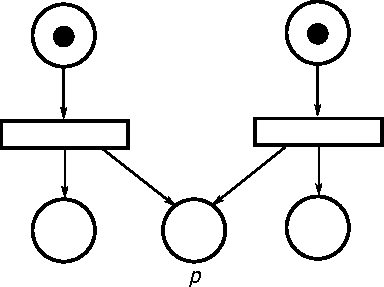
\includegraphics[scale=0.5]{obrazky-figures/PN-parallel2}
		\caption{Ukážka zloženia dvoch sietí. V praxi neužitočné.}
	\end{figure}

	\item Ďaľší prístup je zvážiť ako sa k paralelizmu pristupuje vo výpočetných systémoch. Niekoľko návrhov je schodných. Jeden z najjednoduchších zahŕňa operácie \textbf{FORK} a \textbf{JOIN}. Operácie boli pôvodne navrhnuté Jackom Dennisom a Earlom Van Hornom v roku 1966. Ich prevedenie do Petriho siete je nasledovné: 
	
	\begin{figure}[H]
		\centering
		\begin{minipage}{.4\textwidth}
			\label{fig:fork}
			\centering
			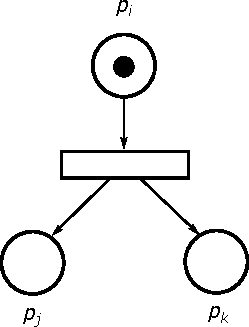
\includegraphics[scale=0.5]{obrazky-figures/PN-fork}
			\caption{Operácia FORK vykonaná v mieste $p_i$ vytvorí proces v miestach $p_j$ a $p_i$.}
		\end{minipage}
	\begin{minipage}{.05\textheight} %spacer
		\quad
	\end{minipage}
		\begin{minipage}{.4\textwidth}
			\label{fig:join}
			\centering
			\includegraphics[scale=0.5]{obrazky-figures/PN-join}
			\caption{Operácia JOIN vykonaná za koncovými miestami procesov $p_j$ a $p_k$ ich spojí a pokračuje v mieste $p_i$.}
		\end{minipage}
	\end{figure}
	
	\item Iný návrh zavedenia paralelizmu je riadiaca štruktúra \textbf{parbegin} a \textbf{parend} [Djikstra 1968]. Koncept navrhnutý Djikstrom má všeobecnú formu $parbegin$ $S_1; S_2;$\dots$S_n$ $parend$, kde $S_i$ predstavuje výraz. Význam $parbegin | parend$ štruktúry je vykonať každý výraz $S_1; S_2;$\dots$S_n$ paralelne. Prevedenie v Petriho sieti je na Obr. \ref{fig:parbegin}.
	
	\begin{figure}[H]
		\centering
		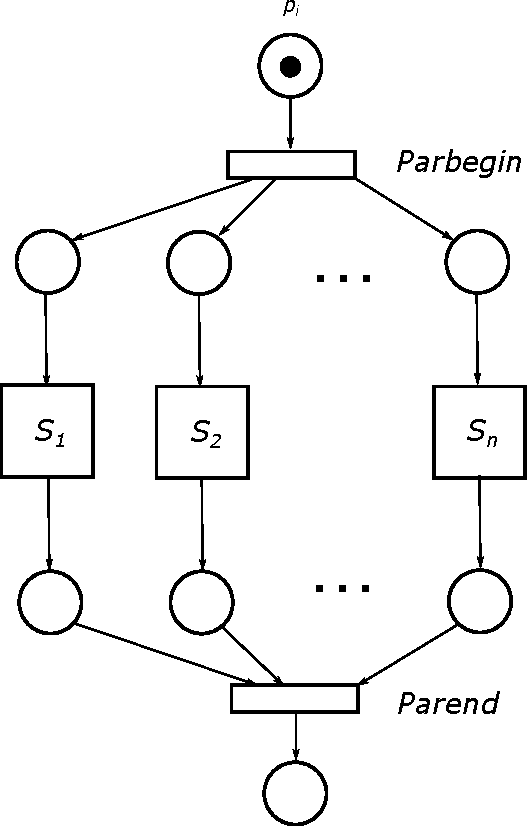
\includegraphics[scale=0.5]{obrazky-figures/PN-parbegin}
		\caption{Riadiaca štruktúra \emph{parbegin} a \emph{parend} v Petriho sieti}
		\label{fig:parbegin}
	\end{figure}
	
	
\end{enumerate} 

\subsection{Čas v Petriho sietiach}

\subsection{Varianty petriho Sietí}
Petriho siete sú koncipované ako plošný (neštrukturovaný) model, kde hierarchický aspekt modelovaného systému nie je nijak vyjadrený. Varianty spomenuté v tejto sekcii sa budú zaoberať rozšírením výpočetnej a modelovacej sily nezbytnej pre prekonanie problému spojeného s plošným statickým modelom. \\\\
\subsubsection{Inhibítory}
Inhibítory umožňujú testovať počet značiek v mieste a tým dávajú Petriho sietiam výpočetnú silu Turingového stroja a sú teda schopné počítať všetky vyčísliteľné funkcie. Takouto sieťou je možné špecifikovat ľubovoľný algoritmus.
\subsubsection{Vysokoúrovňové Petriho siete}
Napriek tomu, že sú siete s inhibítormi schopné vyjadriť akýkoľvek algoritmus, modelovanie čo i len prostého vyhodnocovania aritmetických výrazov je príliš zložité a neintuitívne. Dôvodom sú prostriedky, ktoré zahŕňajú len odjímanie značiek zo vstupných miest a pridávanie značiek do miest výstupných. HL-Siete riešia tento problém zavedením konceptu hranových výrazov, prechodovej stráže a prechodovej akcie.

K tomu, aby sme mohli vysvetliť základné koncepty HL-sítí, potrebujeme pomocný pojem multimnožina a operáciie s multimnožinami.
\begin{defn}
	Majme ľubovolnú neprázdnu množinu $E$. Multimnožina nad množinou $E$ je funkcia. $x : E \longrightarrow \mathbb{N}$. Hodnota $x(e)$ je počet výskytov (koeficient) prvku $e$ v multimnožine $x$. Multimnožinu zapisujeme ako formálnu sumu 
	$$ \sum_{e \in E} x(e)'e $$
	Množinu všetkých multimnožín nad $E$ označíme $E^{MS}$. Pre multimnožiny $x$, $y$ nad $E$ a prirodzené číslo $n$ definujeme:
	
	\begin{enumerate}
		\item sčítanie: $$x + y = \sum_{e \in E} (x(e) + y (e))`e$$
		\item skalárne násobenie: $$n`x = \sum_{e \in E}^{} (n x(e))`e$$
		\item porovnanie:
		$$ x \neq y = \exists e \in E [x(e) \neq y(e) ]$$
		$$ x \leq y = \forall e \in E [x(e) \leq y(e) ]$$
		\item odčítanie: $$x - y = \sum_{e \in E} (x(e) - y (e))`e$$
		\item veľkosť: $$|x| = \sum_{e \in E} x(e)$$
	\end{enumerate}
\end{defn}

\begin{exmpl}
	názorne zápis $2`A + 3`B$ predstavuje multimnožinu s troma výskytmi prvku $a$ a štyrmi výskytmi prvku $b$.
\end{exmpl}

\begin{note}
	Koeficient 1 obvykle vynechávame, tj. napríklad zápis $c$ predstavuje rovnakú multimnožinu ako zápis $1`c$.
\end{note}

Takúto Multimnožinu môžeme konceptom \textbf{hranových výrazov} priradiť k hranám vstupným ako aj výstupným. Názorná ukážka je na Obr. \ref{fig:edge-expr}.

\begin{figure}[H]
	\centering
	\begin{subfigure}[t]{0.4\textwidth}
		\centering
		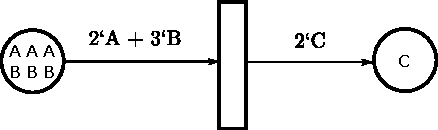
\includegraphics[scale=0.75]{obrazky-figures/PN-edge-expr}
		\caption{Stav pred uskutočnením prechodu}
	\end{subfigure}
	\begin{subfigure}[t]{0.4\textwidth}
		\centering
		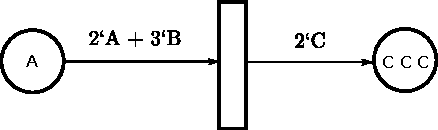
\includegraphics[scale=0.75]{obrazky-figures/PN-edge-exprR}
		\caption{Stav po uskutočnením prechodu}
	\end{subfigure}
	\caption{Hranové výrazy na vstupnej aj výstupnej hrane.}
	\label{fig:edge-expr}
\end{figure}
každému prechodu je možno priradiť \textbf{stráž prechodu}, booleovský výraz, ktorý musí byť splnený pre uskutočnenie prechodu. Je možné určité naviazanie
premenných vo výrazoch na vstupných hranách a rovnako v stráži prechodu. Príklad strážneho výrazu \uv{$x > y$} aj s naväzovaním premenných je na Obr. \ref{fig:guard}.

Pre sugestívnejší zápis dovoluje k stráži prechodu pridať \textbf{akciu prechodu}, odlišujúcu výpočty, ktoré se realizujú pri vykonávaní prechodu, od tých, ktoré se realizujú pri zisťovaní uskutočniteľnosti prechodu.

\begin{figure}[H]
	\centering
	\includegraphics[scale=0.75]{obrazky-figures/PN-guard}
	\caption{Príklad stráže prechodu a akcie prechodu}
	\label{fig:guard}
\end{figure}

\subsubsection{Hierarchické Petriho siete}





\section{PNTalk}

V predošlej kapitole sme sa dozvedeli akú variantu Petriho sietí budeme potrebovať, teraz je na čase predstaviť praktickú implementáciu formalizmu objektovo orientovaných petriho sietí.
\section{Trieda a dedičnosť}

\section{Siete}

\subsection{Objektová sieť}

\subsection{Sieť metód}

\subsection{Sieť konstruktoru}

\subsection{Synchrónny port}

\section{Prechod}

\subsection{Podmienky prechodu}

\subsection{Akcia}

\subsection{Stráž}

\section{PNTalk}

TODO

\chapter{Sekvenčné Diagramy}

Jednou zo štyroch základných modelačných techník UML (Unified Modeling Language) užívanou hojne pri navrhovaní programových systémov je Sekvenčný diagram. Sekvenčný diagram je najbežnejší z kategórie diagramov interakcií a zobrazuje objekty, ktoré sa účastnia v prípade užitia a taktiež zobrazuje správy, ktoré si tieto objekty vymieňajú počas časového intervalu. Diagram je dvojdimenzionálny. Účastníci sú zoradený na horizontálnej ose a časový priebeh je vyjadrený na vertikálnej, kde čas plynie zhora nadol. Ich nespornou výhodou je zobrazovanie aktivity toku správ v časovej postupnosti, to je nápomocné pre porozumenie real-time systémom a komplexným prípadom užitia.

\section{Scenáre}

Sekvenčné diagramy môžu byť generické, zobrazujúce všetky možné scenáre pre definovaný prípad užitia. Častejšie sa však stretneme s vypracovaním diagramov pre jednotlivé scenáre v prípade užitia samostatne.

\section{Komunikácia v sekvenčných diagramoch}

Komunikačný mechanizmus prítomný v sekvenčných diagramoch je, že 
aktivní entity komunikujú priamo, zasielaním správ. 
\begin{note}
	Tu nachádzame konflikt s PT-sieťou v ktorej aktívne entity komunikujú nepriamo, prostredníctvom zdieľaných pasívnych objektov, miestami siete. Mechanizmy sa dajú previesť z jedného na druhý, čo opisuje sekcia :TODO
\end{note}
Sémantika správ je stopa jednoduchej dvojice \lstinline{<sendEvent, RecieveEvent>}, kde \lstinline{sendEvent} je udalosť odoslania správy a \lstinline{recieveEvent} udalosť jej prijatia. Pri absencii jednej udalosti hovoríme o neúplnej správe.

\begin{defn}
	\textbf{Stratená správa} je neúplná správa, pri ktorej je známy výskyt udalosti odoslania správy \lstinline{sendEvent}, ale nie je zaznamenaná udalosť prijatia správy \lstinline{recieveEvent} 
	Typická interpretácia je, že destinácia príjemcu správy je mimo popisovaného rámca. Sémantika je potom zjednodušená na tvar 
	\lstinline{<sendEvent>}.
	Anotácia je šípka vedená od odosielatela zakončená malou bodkou.
\end{defn}

\begin{figure}[H]
	\centering
	\begin{subfigure}[t]{0.4\textwidth}
		\centering
		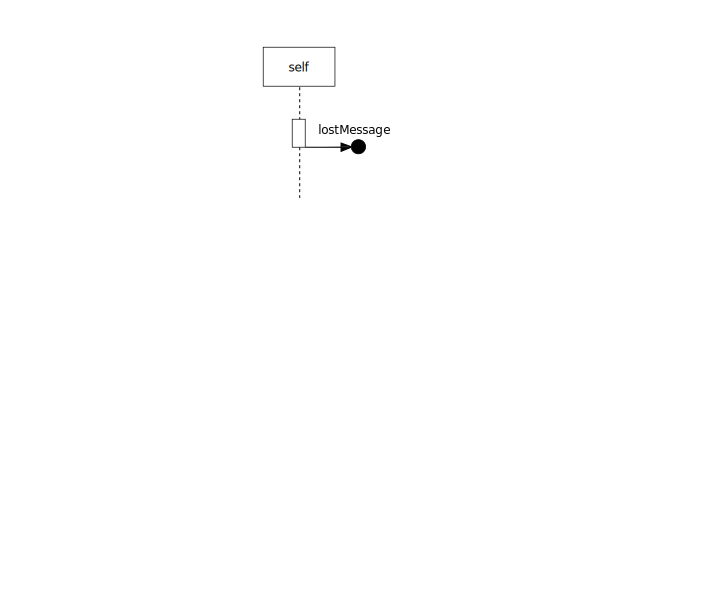
\includegraphics[scale=0.75]{obrazky-figures/SD-lost-ex}
		\caption{Stav pred uskutočnením prechodu}
	\end{subfigure}
	\begin{subfigure}[t]{0.4\textwidth}
		\centering
		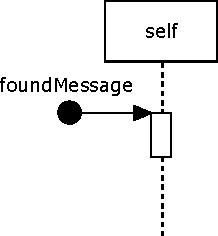
\includegraphics[scale=0.75]{obrazky-figures/SD-found-ex}
		\caption{Stav po uskutočnením prechodu}
	\end{subfigure}
	\caption{Nekompletné správy}
	\label{fig:uncomplete-mes}
\end{figure}

Kompletná správa je v diagrame reprezentovaná orientovanou horizontálnou šípkou smerujúcou od aktívneho objektu odosielateľa k čiare života príjemcu správy. \\\\
V Sekvenčných diagramoch rozlišujeme tri typy správ:

\begin{enumerate}
	\item \textbf{Synchrónna správa} medzi objektami indikuje  sémantiku \emph{wait}, kedy  odosielateľ správy čaká kým je správa spracovaná a pokračuje až po obdržaní odpovede. Správa typicky predstavuje volanie metódy.
	\item \textbf{Asynchrónna správa} používa asynchrónny prístup, pri ktorom nedochádza k žiadnemu blokovaniu objektu odosielateľa. Asynchrónna správa medzi objektami indikuje \emph{no-wait} sémantiku a objekt pokračuje bez toho, aby čakal na odpoveď. Toto dovoľuje paralélne procesy.
	\item \textbf{Odpoveď} predstavuje spätnú správu po synchrónnej správe. Nemôže vzniknúť samostatne.
\end{enumerate}

\begin{figure}[H]
	\centering
	\begin{subfigure}[t]{.3\textwidth}
		\centering
		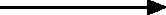
\includegraphics{obrazky-figures/SD-sync}
		\caption{Synchrónna správa}
	\end{subfigure}
	\begin{subfigure}[t]{.3\textwidth}
		\centering
		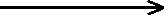
\includegraphics{obrazky-figures/SD-async}
		\caption{Asynchrónna správa}
	\end{subfigure}
\begin{subfigure}[t]{.3\textwidth}
	\centering
	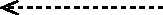
\includegraphics{obrazky-figures/SD-reply}
	\caption{Odpoveď}
\end{subfigure}
	\caption{Reprezentácie troch typov správ}
	\label{fig:arrows}
\end{figure}

\section{Účastníci komunikácie}
Participanti komunikácie skrz správy popísané vyššie sú aktívne objekty, ktoré v sekvenčných diagramoch reprezentujeme čiarou života(\emph{lifeline}).

\begin{defn}
	Pri definícii \textbf{čiary života} začneme netradične notáciou, je zobrazená vertikálnou čiara (môže byť čiarkovaná) predstavujúcu čas života aktívneho objektu. Na jej počiatku sa nachádza hlavička, obdĺžnik obsahujúci \textbf{identifikačnú informáciu} vo formáte: \\
	%\begin{lstlisting}
%<lifelineident> ::= ([<connectable-element-name>[‘[‘ <selector> %‘]’]]
%		[: <connectable-element-type>] [<decomposition>]) | ‘self’
%<selector> ::= <expression>
%<decomposition> ::= ‘ref’ <interactionident> [‘strict’]
%	\end{lstlisting} \vspace{.5cm}
	
	kde \lstinline{<connectable-element-name>} referuje meno typu pripojeného elementu reprezentovaného množinou dodatočných interných datových štruktúr. Napriek tomu, že to zápis dovoľuje \lstinline{<lifelineident>} nemôže byť prázdny.
	
	Ak je identifikátor 'self' čiara života reprezentuje objekt klasifikátoru interakcie, ktorá sama vlastní čiaru života.
	
	
\end{defn} 

\section{Stavebné Elementy sekvenčných Diagramov}

V nasledujúcej sekcii je popísaná syntax a sémantika sekvenčných diagramov.

\subsection{Actor:TODO preklad}

\subsection{objekt}

\subsection{lifeline:TODO preklad čiara života? :D}

\subsection{focus of control:TODO preklad}

\section{Distribuované systémy}

Distribuované systémy majú veľa rozdielnych aspektov, ktoré sa ťažko zachytávajú v jednej difinícii. Je omnoho jednoduchšie hovoriť o distribuovaných systémoch špecifikovaním charakteristík, symptómmi, či média distribúcie. \cite{} V tejto práci budeme mať pod pojmom distribuovaný systém uvažovať systém distribuovaný na počítačovej sieti. \\

Distribúcia prichádza ruka v ruke s vednými disciplínami ako tolerácia chýb, real-time systémy, bezpečnosť a systémový manažment

\subsection{Vymedzenie pojmu distribuovaný systém}

Pred definovaním distribuovaného systému, je vhodné vyjasniť rozdiel s často zameňovaným pojmom počítačových sietí.

\begin{displayquote}
	``Počítačová sieť nie je distribuovaný systém.''
\end{displayquote}

\textbf{Počítačová sieť} je infraštruktúra slúžiaca niekoľkým počítačom  pripojeným k sieti cez komunikačné prepojenie realizované rôznymi médiami a topológiami, a používajú zavedný komunikačný protokol.
Zatiaľ čo \textbf{Distribuovaný systém} je systém pozostávajúci z niekoľkých počítačov, ktoré komunikujú cez počítačovú sieť, hosťujú procesy, ktoré využívajú distribučné protokoly, ktoré zabezpečujú koherentné vykonanie distribuovaných aktivít. \\

\begin{exmpl}
	Vezmime si taký Internet, je to rozsiahla počítačová sieť, vlastne najpodstatnejšia sieť dnes. Používa TCP/IP ako komunikačný protokol.
	Napriek tomu, že tradične poskytuje zopár aplikačných služieb ako e-mail a telnet, nie je to distribuovaný systém. \\
	
	To samozrejme nebráni distribuovaným systémom byť postavených na internete alebo používania internetových technológií, ako distribuované súborové systémy a databázové systémy.
	Jeden z najpodstatnejšįch rozdieľov je, že v prípade distribuovaných systémov procesy zdieľajú spoločný stav a spolupracujú na dosiahnutí spoločného cieľu. Narozdiel od procesov v tomto príklade, ktoré nemusia spolupracovať, len si napríklad vymieňať správy (ako e-mail) bez spoločného cieľu.
\end{exmpl}

\subsection{Porovnanie s Centralizovanými systémami}

V Tabuľke \ref{Tab:central_vs_distr} sú zaznamenané vlastnosti v porovanní s centrálnym systémom ako protipólom k distribuovanému systému. Poznanie rozdieľov, výhod a nevýhod oboch systémov je kľúčové pri návrhu systému. Na základe týchto informácií sa možno ľahšie rozhodnúť, ktorú variantu zvoliť.

\begin{table} [ht]
\begin{center}
	\begin{tabular}{| c | c |} 
		\hline
		Centralizované systémy & Distribuované systémy \\ [0.5ex] 
		\hline\hline
		Dostupnosť & Geografický rámec \\ 
		Homogenita & Heterogenita \\
		Spravovateľnosť & Modularita \\
		 & Škálovateľnosť \\
		 Konzistencia & Zdieľanie \\
		 & Pozvoľná degradácia \\
		 Bezpečnosť & Bezpečnosť \\
		 & Finančný faktor \\ [1ex] 
		\hline
	\end{tabular}
\end{center}
\caption{Porovnanie centralizovaných a distribuovaných systémov}
\label{Tab:central_vs_distr}
\end{table}

Centralizované systémy prirodzene prichádzajú s ľahkou \textbf{dostupnosťou} zdrojov a informácii systému, keďže sú lokálne dostupné. Na druhú stranu Distribuované systémy majú potencionálne \textbf{široký geografický rámec}, preto prístup k zdrojom je niekedy možný len cez vzdialené procedurálne volania.

 \textbf{Homogenita} technológií a procedúr je charakteristická pre centralizované systémy, čím sa myslí jeden operačný systém pre celý systém, ťažké odklonenie sa od používaných technológií systému (programovací jazyk, aplikační rámec). Kdežto u distribuovaných systémov je podporovaná \textbf{heterogenita}, ktorá dovoľuje mať pre každú komponentu odlišné prostredie. Homogenita zjednodušuje správu centrálnych systémov. Heterogenita činí distribuovaný systém inkrementálne rozšíriteľný, ikeď centralizované systémy môžu s dodržaním homogenity dosiahnuť rovnaké rozmery. Skutočná výhoda je až pri \textbf{škálovateľnosti}, kedy centralizované systémy môžu škálovať len \textbf{vertikálne}, to jest zlepšovať výkon nahradzovaním hardvéru za výkonnejší na svojej jednej centrálnej inštancii. Takéto škálovanie je obmedzené technológiou, hardvér sa nedá zlepšovať do nekonečna. Pri distribuovanom systéme máme možnosť škálovať \textbf{horizontálne}, obsluhovať dosiahnutie spoločného cieľu na viacerých inštanciách zároveň. Rozdieľ medzi vertikálnym a horizontálnym škálovaním je graficky znázornený na obrázku \ref{fig:scaling}. 

\begin{figure}[H]
	\centering
	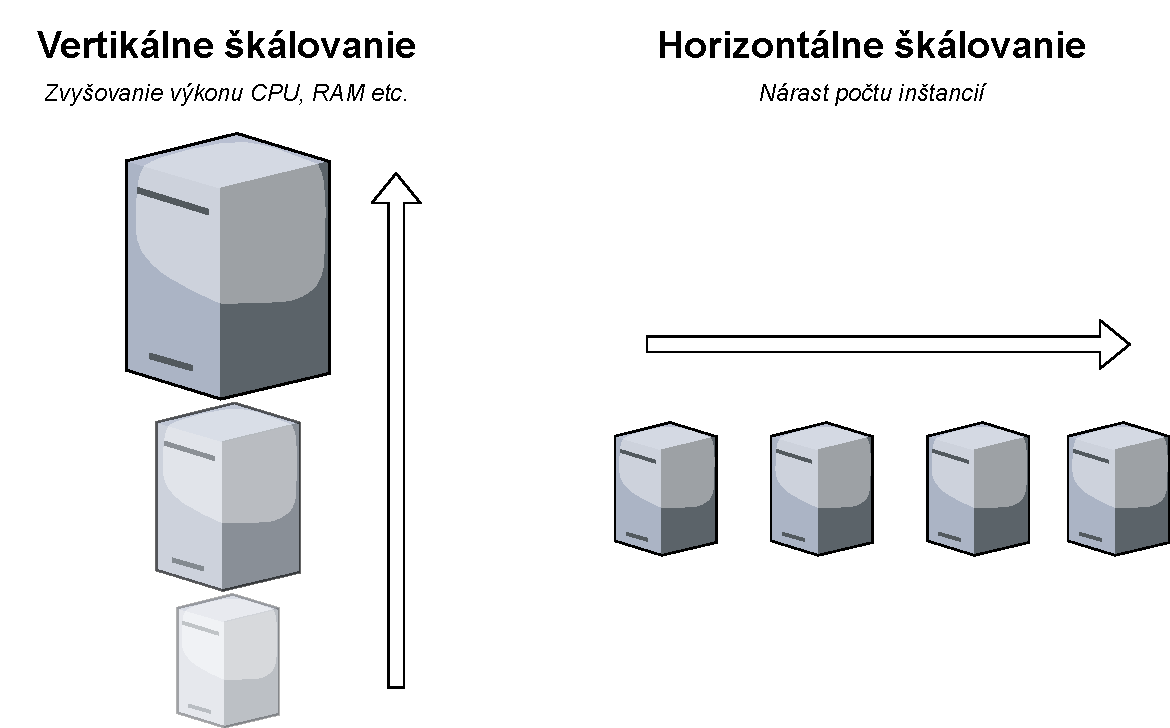
\includegraphics[scale=0.6]{obrazky-figures/TR-scaling}
	\caption{Vertikálne a horizontálne škálovanie}
	\label{fig:scaling}
\end{figure}

\textbf{Konzistenciu} ľahšie dosiahneme u centralizovaných systémov, u distribuovaných je obtiažnejšie zachytiť globálny stav naprieč širokým globálnym rámcom všetkých komponent. \textbf{Pozvoľná degradácia} je vlastnosť systému, ktorý beží kontinuálne spôsobom opatrujúcim možnosť zlyhania komponenty spôsobom, ktorý predíde zlyhaniu celého systému. Tu možno pozorovať silu distribučného systému, kedy pri zlyhaní menšej časti je systém stále dostupný vďaka vysporiadavaniu sa s chybami. Navyše je nepravdepodobné zlyhanie všetkých komponent v rovnaký čas kvôli geografickej separácii jednotlivých komponent.

\textbf{Bezpečnosť} sa dosahuje ľahšie u izolovaného systému s fyzickým prístupom. To nie je možné u distribuovaného systému, avšak vysoká miera bezpečnosti sa dá zaistiť zameraním sa na redukovanie negatívneho efektu vniknutia do systému, než redukovaním hrozieb vzniku neoprávneného vniknutia.

Shrnutím vidíme, že výhody značne prevyšujú ak sa správne rozhodneme, kedy je potreba systém distribuovať.

\subsection{Kedy distribuovať}


Keď nepotrebujeme distribuovaný systém, tak zásadne nedistribujeme. Zbytočne by sme si tým skomplikovali život. Odpoveď pozostáva z troch esenciálnych príčin prečo distribuovať

\begin{enumerate}
	\item Keď má riešený problém decentralizovanú podstatu \\
	\begin{exmpl}
		Zriadujeme systém používajúci konkurenntné procesy na zdrojoch vzdialených pobočiek.
	\end{exmpl}
	\item Keď techniky distribúcie sú vhodnou súčasťou riešenia \\
	\begin{exmpl}
		Systém banky, ktorá potrbuje zálohovať a synchronizovať dáta v dvoch geograficky odľahlých miestach
	\end{exmpl}
	\item Keď problém predpokladá časté zmeny a evolúciu funkcionality, či presunu geografickej polohy. \\
	\begin{exmpl}
		Systém prepožičiavania výpočetných zdrojov medzi vzdialenými uživateľmi.
	\end{exmpl}
\end{enumerate}

\section{Vývojové prostredie}
	Táto kapitola sa zaoberá rozborom vývojových prostredí a ich dekompozíciou na jednotlivé editory a grafické nástroje prítomné v úspešných vývojových prostrediach. \\
	
	Ich význam spočíva v uľahčení práce programátora, zefektívnením kódovania a rýchelho detekovania problémov. Prostredie vedie programátora cez proces editovania, kompilácii či interpretovania kódu a odľaďovania(debugging).
	
	\subsection{Projektový pohľad}
	Predtým než sa pustíme do editovania kódu, musí vývojové prostredie naviazať spojenie s operačným systémom a jeho súborovým systémom. Pri otvorení projektu sken koreňového adresára nahrá do vývojového prostredia kópie súborov a zobrazí ich graficky v projektovom pohľade. Väčšinou je na grafickom uživateľskom rozhraní zobrazovaný pomocou hierarchického stromu, kde listy sú súbory projektu a uzly sú adresáre.
	
	\begin{figure}[H]
		\label{fig:ui-project-pane}
		\centering
		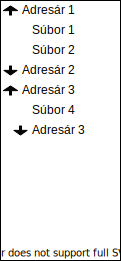
\includegraphics[scale=0.75]{obrazky-figures/UI-project-pane}
		\caption{Ukážka projektového pohľadu s využitím stromovej štruktúry}
	\end{figure}
	
	
	\subsection{Editor zdrojového kódu}
	\label{sec:TR-code-editor}
	Neoddeliteľnou súčasťou každého vývojového prostredia je editor zdrojového kódu, ktorý urýchľuje tvorenie validného kódu v danom programovacom jazyku (väčšina vývojových prostredí má len jeden) za pomoci funkcionalít ako:
	\begin{enumerate}
		\item \textbf{našepkávanie kódu}
		\item \textbf{zvýrazňovanie kľúčových slov}
		\item \textbf{vyhľadávanie a nahradzovanie v kóde}
	\end{enumerate}

	Existuje ich omnoho viac, záleží na konkrétnej implementácii a programovacieho jazyka.
	
	\subsection{Preklad}
	Preklad vo vývojovom prostredí neprebieha na príkazovej riadke, ale odoslanie zdrojových kódov prekladaču alebo interpretu v prípade interpretovaných jazykov je schované v rozhraní za prívetivejšiu variantu tlačítka alebo klávesovej skratky.
	
	\subsection{Ladenie}
	Detekovanie chyby v kóde sa urýchly, ak nám vývojové prostredie umožní kód krokovať, zastaviť a v ktorom koľvek bode sledovať stav premenných.



\chapter{Návrh Implementácie}

Základná myšlienka samotného prevádzania objektovo orientovaných petriho sietí je využiť diskrétnu simuláciu tejto siete, ktorej kroky nám vytvoria časové kontinuum inak chýbajúce v petriho sietiach. 

\section{Architektúra}

Generátor sekvenňých diagramov\cite{Analysis2012} je priamo závislý na dvoch komponentách, validátorom kódu jazyka PNTalk a simulátoru objektovo orientovaných Petriho sietí. Je dôležité zvážiť napojenie týchto komponent ku genrátoru. Vzhľadom k rozličným vlastnostiam jednotlivých implementácii bola motivácia navrhnúť distribuovaný systém s externými komponentami. V generátore uviesť cestu k spustiteľnému binárnemu kódu, ktorého výstup odpovedá definovanému rozhraniu. Daný scenár je uplatniteľný ak pre generátor chceme vyvýjať aj vlastný simulátor, či validátor kódu. V opačnom prípade je vhodnejšie spúšťať externé mikro služby ako webové aplikácie s znovu s vyhradeným komunikačným rozhraním. Pri tejto variante sa namiesto cesty k binárnemu kódu udá generátoru len url adresa webovej aplikace. Tým sa odstráni nechcená závislosť na externej komponente, ktorej pamäťová náročnosť môže presiahnuť pamäťovú náročnosť samotného generátora.

Samotné dáta, prúdiace medzi komponentami, či už vo variante lokálne preloženej binárky, alebo webovej aplikácie musia dodržovať jednotné rozhranie a musia byť serializované zo zrejmých príčin. Pri výbere serializačného formátu je nutno zvážiť viaceré faktory ako podpora v rozličných programovacích jazykoch, ľudsky čiteľnejšie textovo založené formáty alebo binárne uložené dáta, ktoré síce postrádajú ľudskú čiteľnosť no vyžadujú menej pamäte a aj ich zápis a čįtanie je časovo menej náročné. Binárne serializačné formáty by zlepšili responsivitu komponent a dáta posielané v ľudsky čiteľnom formáte by mali nespornú výhodu v odľaďovaní programu. Schodnou variantou sa preto javí podpora viacerých formátov prímaných generátorom od ostatným komponent. Nevýhodou je vznik réžie okolo dohadovaní si serializačného formátu medzi komponentami.

\section{Napojenie na existujúce validátory jazyka PNTalk a simulátory Objektovo orientovaných Petriho sietí}



V tejto Kapitole budú prednesené hlavné myšlienky ako vytvoriť základné stavebné jednotky sekvenčného diagramu. Popisujúc odkiaľ čerpať potrebné informácie zo simulácie, ako si poradiť z neúplnými informáciami a ako sa vysporiadať z absenciou potrebnej informácie zo simulácie OOPN aby bola škoda na výsledku generátora, čo najnižšia. Kapitola je úzko spätá s predchádzajúcimi dvoma kapitolami, keďže bude ťažiť z možností formalismu OOPN a zároveň z vyjadrovacích schopností jazyka PNTalk na vytvorenie datovej štruktúry pre sekvenčný diagram.

\subsection*{Objekt}
Objekt alebo entita je kľúčová časť v scenáry sekvenčného diagramu. Je to obdĺžnik so štítkom mena vo vnútri v ktorom započne čiara života (lifeline) až do deštrukcie objektu, alebo konca simulácie.

\subsubsection*{Vytvorenie objektu}
Na vytvorenie objektu v sekvenčnom diagrame potrebujeme zo simulácie archivovať minimálne 3 veci:

\begin{enumerate}
	\item čas simulácie v ktorom sa inštancia vytvorí
	\item inštanciu, ktorá inicializovala vytvorenie
	\item triedu vytváranej inštancie
\end{enumerate}
Vďaka týmto údajom sa dá vytvoriť správa v sekvenčnom diagrame, ktorá odsadí objekt vertikálne od počiatku do vzdialenosti podľa času vytvorenia.\\\\
\textit{Poznámka: dodatočne sa bude archivovať aj miesto, kam sa objekt uloží pre počítanie referencií. To sa uplatní pri deštrukcii objektu.}


\subsubsection*{Deštrukcia objektu}
Pre deštrukciu objektu musí zaniknúť posledná referencia na objekt. Kvôli tomu je potreba počítadlo referencií, ktoré však nebude výkonnostne náročné ako plnohodnotný garbage collector. Vďaka selektívnemu výberu prechodov, ktoré manipulujú s miestami, kde sú uložené objekty môžme zredukovať počet opakovaní algoritmu len na vybrané prechody.
\pagebreak

Prechod môže spôsobiť tri veci pri manipulácii s referenciou:
\begin{enumerate}
	\item presunúť referenciu do iného miesta\\
	Pri presune referencie sa len pozmení záznam miesta, v ktorom sa nachádza.
	\item zduplikovať referenciu do iného miesta\\
	Pri zduplikovaní sa vytvorí nový záznam o referencii.
	\item vymazať referenciu \\
	Pri vymazaní sa skontroluje, či nie je počet referencií na objekt nulový. Ak áno, objekt sa deštruuje volaním správy destruct z inštancie s prechodom, ktorý poslednú referenciu vymazal.
\end{enumerate}


\subsubsection*{Konvencia mena}

Objekty v sekvenčných diagramoch sa pomenúvavajú pomocou nasledujúcej konvencie "meno inštancie:meno triedy" vďaka čomu môžu vzniknúť tri typy objektov:


\begin{minipage}[c]{0.45\textwidth}
\begin{enumerate}
	\item Pomenovaný objekt
	\item Anonymný objekt
	\item objekt neznámej triedy
\end{enumerate}
\end{minipage}
\hfill
\begin{minipage}[c]{0.8\textwidth}
	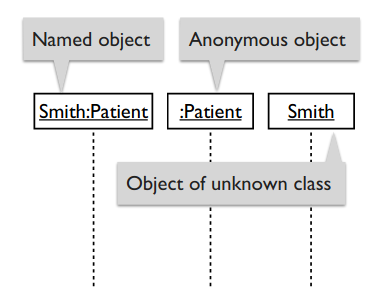
\includegraphics[width=0.45\textwidth]{obrazky-figures/names}
\end{minipage}


syntax jazyka PNTalk vytvára novú inštanciu následovne:

var := classname new.

kde var je dočasná premenná alebo miesto a classname je meno triedy. Problém je zjavný a to, že chýba akákoľvek informácia o mene inštancie. To nám hneď vylúči tretiu možnosť, pretože meno triedy je vždy známe. Varianty sú teda dve a to buď poskladať meno inštancie pomocou známych veličín ako názov miesta, meno triedy, krok simulácie či vygenerovať identifikačné číslo. Druhá varianta je uspokojiť sa s vedomím, že budú vznikať len Anonymné objekty bez názvu inštancie.

\subsection*{Čiara života}
Čiara života alebo inak lifeline je vertikálna čiara reprezentujúca život objektu začína pre každý objekt v dobe vytvorenia a končí deštrukciou objektu, alebo na konci simulácie. Jej vytvorenie je triviálne pokiaľ dokážeme určiť čas vytvorenia a zániku objektu. TODO ref

Je prekrytá bielym obdĺžnikom po dobu, kedy sa metóda objektu nachádza na zásobníku.

\subsubsection*{Na zásobníku}
Doba simulácie po ktorú sa prevádza metóda objektu je viazaná s volaním metód cudzích objektov a preto je nutno archivovať prechody a inštancie, ktoré ich vlastnia. Na tieto prechody potom namapovať prevádzané inštrukcie v chronologickom poradí.

\subsection*{Správa}
Správa vyžaduje poznať odosielateľa, príjemcu a hlavne o aký typ správy sa jedná. Poznáme tri typy:

Synchrónna
Asynchrónna
Odpoveď

zo syntaxe volania metódy pre cudzí objekt evidentne dokážeme zo simulácie odvodiť odosielateľa aj príjemcu.

var methodname: params

kde var je premenná s premennou nesúcou informáciu o mieste s objektom príjemcu. methodname je názov volanej metódy triedy príjemcu. params sú parametre metódy.

odosielateľ je inštancia, ktorá túto akciu zapríčinila svojim prechodom.

Ak metóda vracia hodnotu v simulácii je archivovaná ako odpoveď na správu nesúca údaje o správe na ktorú odpovedá a celú odpoveď.

TODO: Sync vs Async

\subsection*{Cyklus}

K odstráneniu redundantných scenárov značne pomôže zapúzdrenie cyklov, vždy hľadáme v prechodoch najmenší možný ohraničený celok, ktorý sa za sebou sekvenčne niekoľko krát opakuje.

\subsection*{Referovanie a prepájanie diagramov}
Podobne ako pri cykle hľadáme rovnaké, či podobné ohraničené sekvencie prechodov opakujúce sa v simulácii.

\section{Out-source simulácie}

Pre simuláciu bude generátor využívať jeden zo simulátorov objektovo orientovaných petriho sietí z variant bližšie špecifikovaných v kapitole :TODO: . Ako najschodnejšia varianta je zvolený pre túto prácu :TODO: . Aby sme si neuzavreli definitívne dvere k iným implementáciám simulátoru jazyka PNTalk je príhodné zamyslieť sa nad napojením generátoru na simulátor. 

\begin{enumerate}
	\item Varianta pridania kódovej časti do generátoru zjavne možná nie je z dôvodu rôznych implementačných jazykov. Voľba kotlinu ako implementačného jazyka je odôvodnená v sekcii :TODO: .
	
	\item Ponúka sa možnosť vytvoriť dynamickú knižnicu a volať funkcie simulátora z nej. Určite je táto možnosť schodné riešenie, ikeď tu doplácame na neschopnosť preložiť simulátor na všetkých platformách.
	
	\begin{note}
		Linuxová dynamická knižnica *.so nie je ekvivalentná s windowsovou *.dll
	\end{note}
	
	\item Veľmi podobné riešenie je spustiť binárny kód simulátoru s argumentami cestou ku kódu v jazyku PNTalk a zachytením výstupu cout. Oproti predchádzajúcej varianty, vyžaduje omnoho menej úprav.
	
	\item Posledná a taktiež zvolená varianta je pojať generátor ako distribuovaný systém :TODO: , ktorý bude k simulácii využívať komponentu simulátora s ktorou bude komunikovať vopred známym protokolom. To, že si komponenta simulátoru zavolá ďaľšiu komponentu prekladača do medzikódu nebude zo strany generátoru viditeľné. Dôležitý je len pevne daný protokol medzi generátorom a simulátorom, pretože nám to dáva možnosť implementácie simulátoru jednoducho meniť. Stačí aby dodržovali stanovené rozhranie.
	
\end{enumerate}

Distribuovaný systém môže nadobnúť odlišné fyzické formy, či už ide o skupinu osobných počítačov, prepojených lokálnou sieťou, skupinu pracovných staníc zdieľajúcích nielen súborové a databázové systémy, ale navyše aj zdieľaním výpočetnej sily procesora.\cite{}

Distribuovaný systém obsahujúci sadu procesov, ktoré medzi sebou udržujú formu komunikáciu. Okrem konkurenčného behu procesov, niektoré z procesov distribuovaného systému môžu prestať pracovať, pre príklad spadnúť alebo stratiť konektivitu, zatiaľ čo ostatné zostanú bežať a pokračovať v operácii. Toto je podstata čiastočných zlyhaní charakteristických pre distribuované systémy.
\cite{ovilex_ds2016}

\section{Uživateľské rozhranie}

Pri návrhu grafického uživateľského rozhrania je dobré začať položením si otázky "Čo chceme zobrazovať?". Menej je však niekedy viac, pri príliš zložitom rozložení totiž strácame prehľadnosť. \\

\begin{enumerate}
	\item \textbf{Chceme zobraziť momentálne otvorený projekt} \\
	Reprezentáciou by mohol byť hierarchický strom, ktorý by mal v listoch uložené mená súborov a v uzloch mená adresárov. Listy, teda súbory, by mali vizuálnym effektom upozorniť ak je v súbore neuložená zmena. \\
	
	\begin{figure}[H]
		\centering
		\begin{minipage}{.4\textwidth}
			\label{fig:fork}
			\centering
			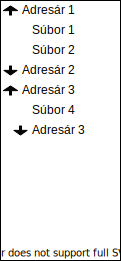
\includegraphics[scale=0.75]{obrazky-figures/UI-project-pane}
			\caption{ Projektový pohľad so schovaným uzlom ``Adresár 2'' a ``Adresár 4''}s
		\end{minipage}
		\begin{minipage}{.05\textheight} %spacer
			\quad
		\end{minipage}
		\begin{minipage}{.4\textwidth}
			\label{fig:join}
			\centering
			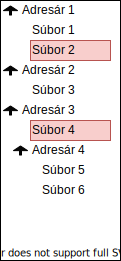
\includegraphics[scale=0.75]{obrazky-figures/UI-project-pane-dirty}
			\caption{Indikácia neuložených zmien v súboroch viditeľná na rozhraní.}
		\end{minipage}
	\end{figure}
	
	\item \textbf{Chceme zobraziť momentálne otvorený súbor s kódom} \\
	Realizujeme to ako editor zdrojového kódu s automatickým zvýrazňovaním kľúčových slov syntaxe jazyka PNTalk a mien z validných definícií. Potrebujeme zobrazovať čísla riadkov.
	\item \textbf{Chceme zobrazovať vygenerovaný diagram} \\
	Potrebujeme na to minimálne rovanko veľa miesta ako na editor zdrojového kódu. Pozadie by malo byť kontrastné vôči diagramu. Celá časť musí byť interaktívna, jednak kvôli pohybu a približovaniu diagramu v okne. Diagram by mal slúžiť ako nástroj na ladenie kódu. To znamená, že kliknutia na jednotlivé časti sekvenčného diagramu by mali vyznačiť reprezentáciu v kóde. Označenie správ by zasa malo zobraziť zmenu miest OOPN, ktoré prechody vyvolali. Označenie, ktoréhokoľvek miesta na čiare života by malo ukázať aktuálne hodnoty v miestach danej inštancie.
	\item \textbf{Chceme zobrazovať posledných \textit{x} riadkov logov}
	Je fajn dať uživateľovi vedieť čo sa deje formou správ, či už chybových alebo informačných. Správy sa musia dať kopírovať a musia byť viditeľné od najnovšej po najstaršiu.
	\item \textbf{Chceme zbytok funkcionalít ukryť do hornej lišty}
	V hornej lište by mali byť kategoricky roztriedené funkcie, s klávesovými skratkami u tých, u ktorých to dáva zmysel.
\end{enumerate}

\subsection{Rozloženie uživateľského rozhrania}

Nie je treba znovu vynaliezať koleso. Pri návrhu rozloženia elementov uživateľského rozhrania sa preto budeme inšpirovať úspešnými vývojovými prostrediami (Visual Studio, IntelliJ IDEA).
To samozrejme neplatí o netradičnom elemente vykresľujúci sekvenčný diagram, je to časť ktorá zobrazuje výstup a zároveň je to aj interaktívny debugger. Inšpiráciu pre tento element by sme hľadali márne, v bežných vývojových prostrediach sa nič podobné nenachádza.
Ničmenej je rovnako, ak nie viac, dôležitý ako editor zdrojového kódu, preto dostane rovnako veľké miesto. \\

Po zvážení veškerých nárokov na uživateľské rohranie vyšlo z procesu návrhu rozloženie na obr. :TODO:

\begin{figure}[H]
	\label{fig:ui-layout}
	\centering
	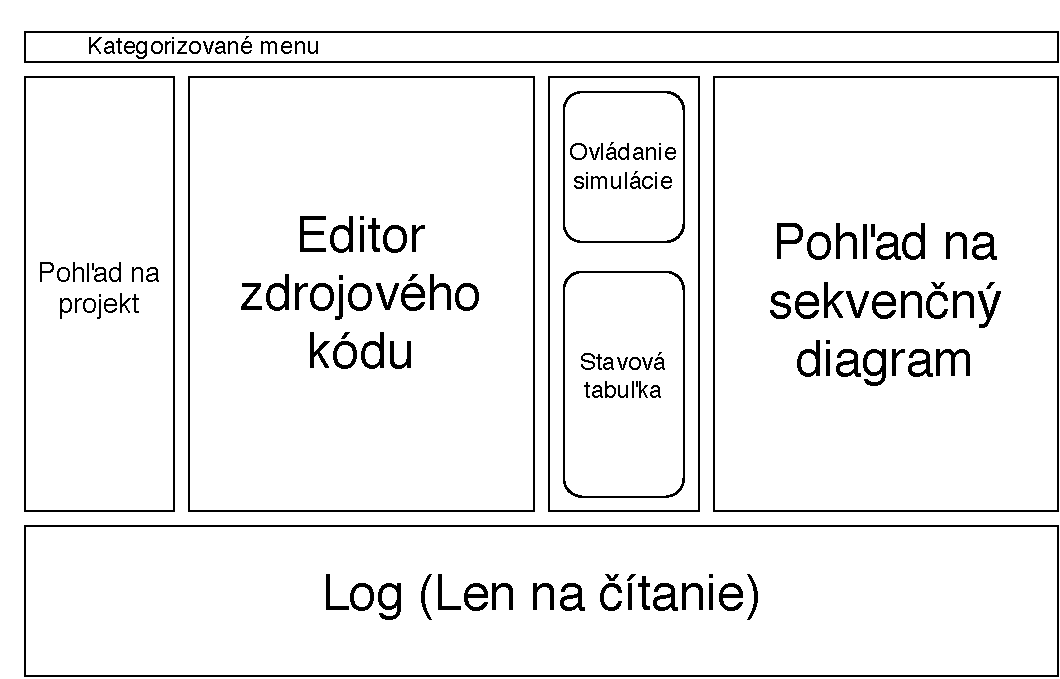
\includegraphics[scale=0.75]{obrazky-figures/UI-layout}
	\caption{Návrh rozloženia grafického uživateľského rozhrania}
\end{figure}



\chapter{Implementácia}

\section{Implementácie distribuovaného systému pomocou Dockeru}

Ako bolo zmienené v návrhu, 

\section{Uživateľské rozhranie}

Implementácia vychádza z dobre pripraveného návrhu v sekcii :TODO: , ktorá bola realizovaná za pomoci kotlinovského aplikačného rámcu TornadoFX nad softvérovou platformou JavaFX.

\subsection{JavaFX v kotline} 

\subsection{Editor Zdrojového kódu}

V sekcii \ref{sec:TR-code-editor} boli vymenované niektoré funkcionality, ktoré nesmú chýbať v moderných editoroch zdrojového kódu. Z nich bolo implementované zvýrazňovanie kľúčových slov jazyka PNtalk a zvýrazňovanie všetkých validne definovaných názvov tried, prechodov, miest, synchrónnych portov a metód.

Zvýrazňovanie zaisťuje asynchrónna funkcia computeHighlighting volaná nad textom z editoru. Je postavená na vyhľadávaní regulárnych výrazov. Globálne v celom rámci sa zvýrazňujú kľúčové slová jazyka PNTalk a mená tried. V rámci danej triedy sa k nim pridá vyhľadávanie názvov prechodov, miest, synchrónnych portov definovaných však len v rozsahu danej triedy.

\chapter{Záver}

Práca demonštroje automatický prevod objektovo orientovaných Petriho sietí na sekvenčné diagramy, generovanie však pokrýva len podmnožinu sekvenčných diagramov. Objekty Actors vystupujúce v konvenčne vytvorených sekvenčných diagramoch sú v práci zanedbané (keďže informáciu na rozlíšenie obyčajných objektov od Actors nedokázali poskytnúť definície v kóde, ani následná simulácia) a Actors preto vystupujú len ako všeobecné objekty. Ďaľší zrejmý nedostatok vyplýva z naviazania na neúplnú implementáciu simulátora, ktorá neumožňuje simuláciu všetkých validných konštrukcií jazyka PNTalk, len ich podmnožinu. Istou kompenzáciou jest architektúra navrhnutá ako distrubovaný systém, ktorá robí tento problém ľahko riešiteľným v budúcnosti po implementovaní vhodnejšej varianty simulátora. Na Záver je vhodné položiť si otázku či sme boli úspešný.
To nám zodpovie sada validačných testov. Jedná sa o netriviálne Petriho siete zadefinované v jazyku PNTalk, ktorých vygenerované výstupy boli porovnané s tými ručne vytvorenýmí. Okrem validity vzišla motivácia zaznamenať výsledky aj časovej náročnosti. Časová náročnosť sa merala pre samotný proces generácie sekvenčných diagramov ako aj celkovo beh v spolupráci externých komponent. Plán bol vytýčiť hranice, pre ktoré by bolo reálne simulovať a vykreslovať výsledok generácie ihneď pri zmene vstupnęho kódu. Kvôli neuspokojivým výsledkom v tomto teste (:TODO: graf) sa z pokusu o implementácie funkcie "hot-reload" upustilo. 

\section{Výsledky testovania}




 


  \fi
  
  % Kompilace po částech (viz výše, nutno odkomentovat)
  % Compilation piecewise (see above, it is necessary to uncomment it)
  %\subfile{projekt-01-uvod-introduction}
  % ...
  %\subfile{chapters/projekt-05-conclusion}


  % Pouzita literatura / Bibliography
  % ----------------------------------------------
\ifslovak
  \makeatletter
  \def\@openbib@code{\addcontentsline{toc}{chapter}{Literatúra}}
  \makeatother
  \bibliographystyle{bib-styles/Pysny/skplain}
\else
  \ifczech
    \makeatletter
    \def\@openbib@code{\addcontentsline{toc}{chapter}{Literatura}}
    \makeatother
    \bibliographystyle{bib-styles/Pysny/czplain}
  \else 
    \makeatletter
    \def\@openbib@code{\addcontentsline{toc}{chapter}{Bibliography}}
    \makeatother
    \bibliographystyle{bib-styles/Pysny/enplain}
  %  \bibliographystyle{alpha}
  \fi
\fi
  \begin{flushleft}
  \bibliography{projekt-20-literatura-bibliography}
  \end{flushleft}

  % vynechani stranky v oboustrannem rezimu
  % Skip the page in the two-sided mode
  \iftwoside
    \cleardoublepage
  \fi

  % Prilohy / Appendices
  % ---------------------------------------------
  \appendix
\ifczech
  \renewcommand{\appendixpagename}{Přílohy}
  \renewcommand{\appendixtocname}{Přílohy}
  \renewcommand{\appendixname}{Příloha}
\fi
\ifslovak
  \renewcommand{\appendixpagename}{Prílohy}
  \renewcommand{\appendixtocname}{Prílohy}
  \renewcommand{\appendixname}{Príloha}
\fi
%  \appendixpage

% vynechani stranky v oboustrannem rezimu
% Skip the page in the two-sided mode
%\iftwoside
%  \cleardoublepage
%\fi
  
\ifslovak
%  \section*{Zoznam príloh}
%  \addcontentsline{toc}{section}{Zoznam príloh}
\else
  \ifczech
%    \section*{Seznam příloh}
%    \addcontentsline{toc}{section}{Seznam příloh}
  \else
%    \section*{List of Appendices}
%    \addcontentsline{toc}{section}{List of Appendices}
  \fi
\fi
  \startcontents[chapters]
  \setlength{\parskip}{0pt} 
  % seznam příloh / list of appendices
  % \printcontents[chapters]{l}{0}{\setcounter{tocdepth}{2}}
  
  \ifODSAZ
    \setlength{\parskip}{0.5\bigskipamount}
  \else
    \setlength{\parskip}{0pt}
  \fi
  
  % vynechani stranky v oboustrannem rezimu
  \iftwoside
    \cleardoublepage
  \fi
  
  % Přílohy / Appendices
  \ifenglish
    \input{projekt-30-prilohy-appendices-en}
  \else
    % Tento soubor nahraďte vlastním souborem s přílohami (nadpisy níže jsou pouze pro příklad)

% Umístění obsahu paměťového média do příloh je vhodné konzultovat s vedoucím
%\chapter{Obsah přiloženého paměťového média}

%\chapter{Manuál}

%\chapter{Konfigurační soubor}

%\chapter{RelaxNG Schéma konfiguračního souboru}

%\chapter{Plakát}

\chapter{Jak pracovat s touto šablonou}
\label{jak}

V této příloze je uveden popis jednotlivých částí šablony, po kterém následuje stručný návod, jak s touto šablonou pracovat. Pokud po jejím přečtení k šabloně budete mít nějaké dotazy, připomínky apod., neváhejte a napište na e-mail \texttt{sablona@fit.vutbr.cz}.

\section*{Popis částí šablony}

Po rozbalení šablony naleznete následující soubory a adresáře:
\begin{DESCRIPTION}
  \item [bib-styles] Styly literatury (viz níže). 
  \item [obrazky-figures] Adresář pro Vaše obrázky. Nyní obsahuje \texttt{placeholder.pdf} (tzv. TODO obrázek, který lze použít jako pomůcku při tvorbě technické zprávy), který se s prací neodevzdává. Název adresáře je vhodné zkrátit, aby byl jen ve zvoleném jazyce.
  \item [template-fig] Obrázky šablony (znak VUT).
  \item [fitthesis.cls] Šablona (definice vzhledu).
  \item [Makefile] Makefile pro překlad, počítání normostran, sbalení apod. (viz níže).
  \item [projekt-01-kapitoly-chapters.tex] Soubor pro Váš text (obsah nahraďte).
  \item [projekt-20-literatura-bibliography.bib] Seznam literatury (viz níže).
  \item [projekt-30-prilohy-appendices.tex] Soubor pro přílohy (obsah nahraďte).
  \item [projekt.tex] Hlavní soubor práce -- definice formálních částí.
\end{DESCRIPTION}

Styl literatury v šabloně je od Ing. Radka Pyšného \cite{Pysny}, jehož práce byla vylepšena prof. Adamem Heroutem, dr. Jaroslavem Dytrychem a panem Karlem Hanákem tak, aby odpovídala normě a podporovala všechny často využívané typy citací. Jeho dokumentaci naleznete v příloze \ref{priloha-priklady-citaci}.

\begin{samepage}
Makefile kromě překladu do PDF nabízí i další funkce:
\begin{itemize}
  \item přejmenování souborů (viz níže),
  \item počítání normostran,
  \item spuštění vlny pro doplnění nezlomitelných mezer,
  \item sbalení výsledku pro odeslání vedoucímu ke kontrole (zkontrolujte, zda sbalí všechny Vámi přidané soubory, a případně doplňte).
\end{itemize}
\end{samepage}

Nezapomeňte, že vlna neřeší všechny nezlomitelné mezery. Vždy je třeba manuální kontrola, zda na konci řádku nezůstalo něco nevhodného -- viz Internetová jazyková příručka\footnote{Internetová jazyková příručka \url{http://prirucka.ujc.cas.cz/?id=880}}.

\paragraph {Pozor na číslování stránek!} Pokud má obsah 2 strany a na 2. jsou jen \uv{Přílohy} a~\uv{Seznam příloh} (ale žádná příloha tam není), z nějakého důvodu se posune číslování stránek o 1 (obsah \uv{nesedí}). Stejný efekt má, když je na 2. či 3. stránce obsahu jen \uv{Literatura} a~je možné, že tohoto problému lze dosáhnout i jinak. Řešení je několik (od~úpravy obsahu, přes nastavení počítadla až po sofistikovanější metody). \textbf{Před odevzdáním proto vždy překontrolujte číslování stran!}


\section*{Doporučený postup práce se šablonou}

\begin{enumerate}
  \item \textbf{Zkontrolujte, zda máte aktuální verzi šablony.} Máte-li šablonu z předchozího roku, na stránkách fakulty již může být novější verze šablony s~aktualizovanými informacemi, opravenými chybami apod.
  \item \textbf{Zvolte si jazyk}, ve kterém budete psát svoji technickou zprávu (česky, slovensky nebo anglicky) a svoji volbu konzultujte s vedoucím práce (nebyla-li dohodnuta předem). Pokud Vámi zvoleným jazykem technické zprávy není čeština, nastavte příslušný parametr šablony v souboru projekt.tex (např.: \verb|document|\verb|class[english]{fitthesis}| a přeložte prohlášení a poděkování do~angličtiny či slovenštiny.
  \item \textbf{Přejmenujte soubory.} Po rozbalení je v šabloně soubor \texttt{projekt.tex}. Pokud jej přeložíte, vznikne PDF s technickou zprávou pojmenované \texttt{projekt.pdf}. Když vedoucímu více studentů pošle \texttt{projekt.pdf} ke kontrole, musí je pracně přejmenovávat. Proto je vždy vhodné tento soubor přejmenovat tak, aby obsahoval Váš login a (případně zkrácené) téma práce. Vyhněte se však použití mezer, diakritiky a speciálních znaků. Vhodný název může být např.: \uv{\texttt{xlogin00-Cisteni-a-extrakce-textu.tex}}. K přejmenování můžete využít i přiložený Makefile:
\begin{verbatim}
make rename NAME=xlogin00-Cisteni-a-extrakce-textu
\end{verbatim}
  \item Vyplňte požadované položky v souboru, který byl původně pojmenován \texttt{projekt.tex}, tedy typ, rok (odevzdání), název práce, svoje jméno, ústav (dle zadání), tituly a~jméno vedoucího, abstrakt, klíčová slova a další formální náležitosti.
  \item Nahraďte obsah souborů s kapitolami práce, literaturou a přílohami obsahem svojí technické zprávy. Jednotlivé přílohy či kapitoly práce může být výhodné uložit do~samostatných souborů -- rozhodnete-li se pro toto řešení, je doporučeno zachovat konvenci pro názvy souborů, přičemž za číslem bude následovat název kapitoly. 
  \item Nepotřebujete-li přílohy, zakomentujte příslušnou část v \texttt{projekt.tex} a příslušný soubor vyprázdněte či smažte. Nesnažte se prosím vymyslet nějakou neúčelnou přílohu jen proto, aby daný soubor bylo čím naplnit. Vhodnou přílohou může být obsah přiloženého paměťového média.
  \item Smažte soubory s kapitolami a přílohami pro jazyk, který jste nevyužili (s nebo bez \texttt{-en}).
  \item Zadání, které si stáhnete v PDF z IS FIT (odkaz \uv{Zadání pro vložení do práce} či \uv{Thesis assignment}), uložte do souboru \texttt{zadani.pdf} a povolte jeho vložení do práce parametrem šablony v \texttt{projekt.tex} (\verb|document|\verb|class[zadani]{fitthesis}|).
  \item Nechcete-li odkazy tisknout barevně (bez konzultace s vedoucím příliš nedoporučuji), budete pro tisk vytvářet druhé PDF s tím, že nastavíte parametr šablony pro tisk: (\verb|document|\verb|class[zadani,print]{fitthesis}|). Budete-li tisknout barevně, místo \texttt{print} použijte parametr \texttt{cprint}. Barevné logo se nesmí tisknout černobíle!
  \item Vzor desek, do kterých bude práce vyvázána, si vygenerujte v informačním systému fakulty u zadání. Pro disertační práci lze zapnout parametrem v šabloně \texttt{cover} (více naleznete v souboru \texttt{fitthesis.cls}).
  \item Nezapomeňte, že zdrojové soubory i (obě verze) PDF musíte odevzdat na CD či jiném médiu přiloženém k technické zprávě.
\end{enumerate}

Obsah práce se generuje standardním příkazem \tt \textbackslash tableofcontents \rm (zahrnut v šabloně). Přílohy jsou v něm uvedeny úmyslně.

\subsection*{Pokyny pro oboustranný tisk}
\begin{itemize}
\item \textbf{Oboustranný tisk je doporučeno konzultovat s vedoucím práce.}
\item Je-li práce tištěna oboustranně a její tloušťka je menší než tloušťka desek, nevypadá to dobře.
\item Zapíná se parametrem šablony: \verb|\document|\verb|class[twoside]{fitthesis}|
\item Po vytištění oboustranného listu zkontrolujte, zda je při prosvícení sazební obrazec na obou stranách na stejné pozici. Méně kvalitní tiskárny s duplexní jednotkou mají často posun o 1--3 mm. Toto může být u některých tiskáren řešitelné tak, že vytisknete nejprve liché stránky, pak je dáte do stejného zásobníku a vytisknete sudé.
\item Za titulním listem, obsahem, literaturou, úvodním listem příloh, seznamem příloh a případnými dalšími seznamy je třeba nechat volnou stránku, aby následující část začínala na liché stránce (\texttt{\textbackslash cleardoublepage}).
\item  Konečný výsledek je nutné pečlivě překontrolovat.
\end{itemize}

\subsection*{Styl odstavců}

Odstavce se zarovnávají do bloku a pro jejich formátování existuje více metod. U papírové literatury je častá metoda s~použitím odstavcové zarážky, kdy se u~jednotlivých odstavců textu odsazuje první řádek odstavce asi o~jeden až dva čtverčíky, tedy přibližně o~dvě šířky velkého písmene M základního textu (vždy o~stejnou, předem zvolenou hodnotu). Poslední řádek předchozího odstavce a~první řádek následujícího odstavce se v~takovém případě neoddělují svislou mezerou. Proklad mezi těmito řádky je stejný jako proklad mezi řádky uvnitř odstavce \cite{fitWeb}.

Další metodou je odsazení odstavců, které je časté u elektronické sazby textů. První řádek odstavce se při této metodě neodsazuje a mezi odstavce se vkládá vertikální mezera o~velikosti 1/2 řádku. Obě metody lze v kvalifikační práci použít, nicméně často je vhodnější druhá z uvedených metod. Metody není vhodné kombinovat.

Jeden z výše uvedených způsobů je v šabloně nastaven jako výchozí, druhý můžete zvolit parametrem šablony \uv{\tt odsaz\rm }.

\subsection*{Užitečné nástroje}
\label{nastroje}

Následující seznam není výčtem všech využitelných nástrojů. Máte-li vyzkoušený osvědčený nástroj, neváhejte jej využít. Pokud však nevíte, který nástroj si zvolit, můžete zvážit některý z následujících:

\begin{description}
	\item[\href{http://miktex.org/download}{MikTeX}] \LaTeX{} pro Windows -- distribuce s jednoduchou instalací a vynikající automatizací stahování balíčků. MikTex obsahuje i vlastní editor, ale spíše doporučuji TeXstudio.
	\item[\href{http://texstudio.sourceforge.net/}{TeXstudio}] Přenositelné GUI pro \LaTeX{} s otevřeným zdrojovým kódem (opensource).  Ctrl+klik umožňuje přepínat mezi zdrojovým textem a PDF. Má integrovanou kontrolu pravopisu\footnote{Českou kontrolu pravopisu lze doinstalovat z \url{https://extensions.openoffice.org/de/project/czech-dictionary-pack-ceske-slovniky-cs-cz}}, zvýraznění syntaxe apod. Pro jeho využití je nejprve potřeba nainstalovat MikTeX, případně jinou \LaTeX ovou distribuci.
	\item[\href{http://www.winedt.com/}{WinEdt}] Ve Windows je dobrá kombinace WinEdt + MiKTeX. WinEdt je GUI pro Windows, pro jehož využití je nejprve potřeba nainstalovat \href{http://miktex.org/download}{MikTeX} či \href{http://www.tug.org/texlive/}{TeX Live}. 
	\item[\href{http://kile.sourceforge.net/}{Kile}] Editor pro desktopové prostředí KDE (Linux). Umožňuje živé zobrazení náhledu. Pro jeho využití je potřeba mít nainstalovaný \href{http://www.tug.org/texlive/}{TeX Live} a Okular. 
	\item[\href{http://jabref.sourceforge.net/download.php}{JabRef}] Pěkný a jednoduchý program v Javě pro správu souborů s bibliografií (literaturou). Není potřeba se nic učit -- poskytuje jednoduché okno a formulář pro editaci položek.
	\item[\href{https://inkscape.org/en/download/}{InkScape}] Přenositelný opensource editor vektorové grafiky (SVG i PDF). Vynikající nástroj pro tvorbu obrázků do odborného textu. Jeho ovládnutí je obtížnější, ale výsledky stojí za to.
	\item[\href{https://git-scm.com/}{GIT}] Vynikající pro týmovou spolupráci na projektech, ale může výrazně pomoci i jednomu autorovi. Umožňuje jednoduché verzování, zálohování a přenášení mezi více počítači.
	\item[\href{http://www.overleaf.com/}{Overleaf}] Online nástroj pro \LaTeX{}. Přímo zobrazuje náhled a umožňuje jednoduchou spolupráci (vedoucí může průběžně sledovat psaní práce), vyhledávání ve zdrojovém textu či ve vygenerovaném PDF, kontrolu pravopisu apod. Zdarma jej však lze využít pouze s určitými omezeními (někomu stačí na disertaci, jiný na ně může narazit i při psaní bakalářské práce) a pro dlouhé texty je pomalejší. FIT VUT v Brně má pro studenty i~zaměstnance licenci, kterou si lze aktivovat na \url{https://www.overleaf.com/edu/but}.
\end{description}

Pozn.: Overleaf nepoužívá Makefile v šabloně -- aby překlad fungoval, je v menu nutné zvolit \tt projekt.tex \rm jako hlavní dokument.

\chapter{Psaní anglického textu}
\label{anglicky}
Tato příloha je převzata ze stránek doc. Černockého \cite{CernockyEnglish}.

Spousta lidí píše zprávy k projektům anglicky (a to je dobře!), ale dělá v nich spoustu zbytečných chyb (a to je špatně). Nejsem angličtinář, ale tento jazyk už nějakých pár let používám k psaní, čtení i komunikaci -- tato příloha obsahuje pár důležitých věcí. Pokud chcete napsat práci nebo článek opravdu 100\,\% dobře, nezbude Vám než si najmout rodilého mluvčího (a to by měl by být trochu technicky zdatný a aspoň trochu rozumět tomu, co píšete, ať to neskončí ještě hůř \ldots).

\section*{Obecně}

\begin{itemize}
  \item{Předtím, než budete sami něco psát, si přečtěte pár anglických technických článků a~zkuste si zapamatovat a získat \uv{obecný pocit}, jak se to píše.}
  \item{Používejte vždy korektor pravopisu -- zabudovaný ve Wordu, nebo v OpenOffice, pokud děláte na Linuxu, tak ISPELL a další (většina editorů pro \LaTeX{} má již kontrolu pravopisu integrovanou).}
  \item{Používejte korektor gramatiky. Nevím, jestli je nějaký dostupný na Linuxu, ale ten ve Wordu celkem slušně funguje a pokud Vám něco zelené podtrhne, je tam většinou opravdu chyba. Můžete do něj nakopírovat i zdrojový text pro \LaTeX{}, opravit, a pak uložit opět jako čistý text. Pokud používáte vim, je tam zabudovaný také a zvládne jak překlepy, tak základní gramatiku. V dokumentu \texttt{diplomka.tex} na první řádek napište: 
  \begin{verbatim}
    % vim:spelllang=en_us:spell
  \end{verbatim}
  (případně \texttt{en\_gb} pro OED angličtinu)
  \textit{Poznámka editora:} Existuje i velmi dobrý online nástroj Grammarly\footnote{\url{https://www.grammarly.com/}}, který je v základní verzi zdarma. 
  }
  \item{Online slovníky jsou dobré, ale nepoužívejte je slepě. Většinou dají více variant a ne každá je správně.}
  \item{\begin{samepage}Na vyhledávání a zjištění, co bude asi správné, můžete použít Google. Např.: nevíte, jak se řekne \uv{výhoda tohoto přístupu}. Slovník na seznam.cz dá asi 10 variant. Napište je postupně do vyhledávání na googlu:
  \begin{verbatim}
    "advantage of this approach" 1100000 hits
    "privilege of this approach" 6 hits
    "facility of this approach"  16 hits
  \end{verbatim}
  Neříkám, že je to 100\,\% správně, ale je to určité vodítko. Toto se dá použít i~na~dohledání správných spojek (třeba \uv{among two cases} nebo \uv{between two cases}?)\end{samepage}}
\end{itemize}
       
\section*{SVOMPT a shoda}

Struktura anglické věty je SVOPMT: SUBJECT VERB OBJECT MANNER PLACE TIME a přes to nejede vlak! Není volná jako v češtině. Jinak to je maximálně v nějaké divadelní hře, kde je potřeba něco zdůraznit. Hlavně podmět tam musí vždy být, na to se často zapomíná, protože v CZ/SK může být zamlčený nebo nevyjádřený. SVOMPT platí i~ve vedlejších větách!
\begin{verbatim}
  BAD: We have shown that is faster than the other function. 
  GOOD: We have shown that it is faster than the other function. 
\end{verbatim}

\noindent Shoda podmětu s přísudkem -- zní to šíleně, ale dělá se v tom spousta chyb. 

\begin{verbatim}
  he has 
  the users have 
  people were 
\end{verbatim}

\section*{Členy}

Členy v angličtině jsou noční můra a téměř nikdo z nás je nedává dobře. Základní pravidlo je, že když je něco určitého, musí předtím být \uv{the}. Členy musí být určitě u těchto spojení:
\begin{verbatim}
  the first, the second, ...
  the last
  the most (třetí stupeň přídavných jmen a príslovcí) ...
  the whole 
  the following 
  the figure, the table. 
  the left, the right - on the left pannel, from the left to the right ... 
\end{verbatim}

\noindent Naopak člen NESMÍ být, pokud používáte přesné označení obrázku, kapitoly atd.
\begin{verbatim}
  in Figure 3.2
  in Chapter 7
  in Table 6.4
\end{verbatim}

\begin{samepage}
\noindent Pozor na \uv{a} vs. \uv{an}, řídí se to podle výslovnosti a ne podle toho, jak je slovo napsané, takže:
\begin{verbatim}
  an HMM
  an XML
  a universal model
  a user
\end{verbatim}
\end{samepage}

\section*{Slovesa}

Pozor na trpné tvary sloves -- u pravidelných je to většinou bez problémů, u nepravidelných často špatně, typicky
\begin{verbatim}
  packet was sent (ne send)
  approach was chosen (ne choosed)
\end{verbatim}
\noindent \ldots vetšinou to opraví korektor pravopisu, ale někdy ne. 

Pozor na časy, občas je v nich pěkný nepořádek. Pokud něco nějak obecně je, přítomný čas. Pokud jste něco udělali, minulý. Pokud to dalo nějaký výsledek a ten výsledek teď existuje a třeba ho nějak diskutujete, přítomný. Nepoužívejte příliš složité časy jako je předpřítomný a vůbec ne předminulý pokud nevíte přesně, co děláte.
\begin{verbatim}
  JFA is a technique that works for everyone in speaker recognition. 
  We implemented it according to Kenny's recipe in \cite{Kenny}. 
  12000 segments from NIST SRE 2006 were processed. When compared 
  with a GMM baseline, the results are completely bad. 
\end{verbatim}

\section*{Délka vět a struktura}

\begin{itemize}
  \item{Pište kratší věty a souvětí, pokud máte něco na 5 řádků, většinou se to nedá číst.}
  \item{Strukturujte věty pomocí čárek (více než v češtině!), hlavně po úvodu věty, po kterém začíná vlastní věta. Někdy se dává čárka i před \uv{and} (na rozdíl od češtiny).}
\end{itemize}
\begin{verbatim}
  In this chapter, we will investigate ... 
  The first technique did not work, the second did not work as well, 
  and the third one also did not work. 
\end{verbatim}

\section*{Specifika technického textu}

Píšete technický text, proto nepoužívejte zkratky
\begin{verbatim}
  he's
  gonna
  Petr's working on ...
\end{verbatim}
\noindent a podobně. Jediné, které je tolerované, je \uv{doesn't}, ale neuděláte chybu, když napíšete \uv{does not}. 

\begin{samepage}
\noindent V technických textech se spíš používá trpný rod než činný: 
\begin{verbatim}
  BAD: In this chapter, I describe used programming languages. 
  GOOD: In this chapter, used programming languages are described.
\end{verbatim}
\end{samepage}

Pokud už činný použijete, dává se v technických textech spíše \uv{we}, i když na práci děláte sami. \uv{I}, \uv{my} atd. se používají pouze tam, kde jde o to zdůraznit, že jde o Vaši osobu, tedy třeba v závěru nebo v popisu \uv{original claims} v disertaci.

\paragraph{Časté chyby ve slovech}

\begin{itemize}
  \item{Pozor na jeho/její, není to it's, ale its.}
  \item{Obrázek není picture, ale figure. }
  \item{Spojka \uv{než} je \uv{than}, ne \uv{then} -- bigger than this, smaller than this \ldots hrozně častá chyba! \uv{Then} je pak, potom.}
\end{itemize}


\chapter{Checklist} 
\label{checklist}
Tento checklist byl převzat ze šablony pro kvalifikační práce, která je k dispozici na blogu prof. Herouta \cite{Herout}, který s laskavým dovolením využil nápadu dr. Szökeho%
\footnote{\url{http://blog.igor.szoke.cz/2017/04/predstartovni-priprava-letu-neni.html}}. 

Velká bezpečnost letecké dopravy stojí z části na tom, že lidé kolem letadel mají \textbf{checklisty} na úplně každý, třeba rutinní a dobře zažitý, postup. Jako pilot strpí to, že bude trochu za blbce a opravdu tužtičkou do seznamu úkonů odškrtá dokonale zvládnuté akce, vytiskněte si a odškrtejte před odevzdáním diplomky i vy tento checklist a vyhněte se tak častým chybám, které by mohly mít až fatální následky na výsledné hodnocení Vaší práce.

\subsubsection*{Struktura}
\begin{checklist}
	\item Už ze samotných názvů a struktury kapitol je patrné, že bylo splněno zadání.
	\item V textu se nevyskytuje kapitola, která by měla méně než čtyři strany (kromě úvodu a závěru). Pokud ano, radil(a) jsem se o tom s vedoucím a ten to schválil.
\end{checklist}

\subsubsection*{Obrázky a grafy}
\begin{checklist}
	\item Všechny obrázky a tabulky byly zkontrolovány a jsou poblíž místa, odkud jsou z textu odkazovány, takže nebude problém je najít.
	\item Všechny obrázky a tabulky mají takový popisek, že celý obrázek dává smysl sám o~sobě, bez čtení dalšího textu. Vůbec nevadí, když má popisek několik řádků.
	\item Pokud je obrázek převzatý, tak je to v popisku zmíněno: \uv{Převzato z [X].}
	\item Písmenka ve všech obrázcích používají font podobné velikosti, jako je okolní text (ani výrazně větší, ani výrazně menší).
	\item Grafy a schémata jsou vektorově (tj. v PDF).
	\item Snímky obrazovky nepoužívají ztrátovou kompresi (jsou v PNG).
	\item Všechny obrázky jsou odkázány z textu.
	\item Grafy mají popsané osy (název osy, jednotky, hodnoty) a podle potřeby mřížku.
\end{checklist}

\subsubsection*{Rovnice}
\begin{checklist}
	\item Identifikátory a jejich indexy v rovnicích jsou jednopísmenné (kromě nečastých zvláštních případů jako $t_\mathrm{max}$).
	\item Rovnice jsou číslovány.
	\item Za (nebo vzácně před) rovnicí jsou vysvětleny všechny proměnné a funkce, které zatím vysvětleny nebyly.
\end{checklist}

\subsubsection*{Citace}
\begin{checklist}
    \item \textbf{Všechny použité zdroje jsou citovány.}
	\item Adresy URL odkazující na služby, projekty, zdroje, github apod. jsou odkazovány pomocí \verb|\footnote{\url{...}}|.
    \item Všechny citace používají správné typy.
	\item Citace mají autora, název, vydavatele (název konference), rok vydání.  Když některá nemá, je to dobře zdůvodněný zvláštní případ a vedoucí to odsouhlasil.
	\item Je-li ve zdrojových textech programu něco převzaté, je to tam řádně citováno v souladu s licencí.
	\item Je-li podstatná část zdrojových textů programu převzatá, je toto zmíněno v textu práce a je citován zdroj.
\end{checklist}

\subsubsection*{Typografie}
\begin{checklist}
	\item Žádný řádek nepřetéká přes pravý okraj.
	\item Na konci řádku nikde není jednopísmenná předložka (spraví to nedělitelná mezera $\sim$).
	\item Číslo obrázku, tabulky, rovnice, citace není nikde první na novém řádku (spraví to nedělitelná mezera $\sim$).
	\item Před číselným odkazem na poznámku pod čarou nikde není mezera (to jest vždy takto\footnote{příklad poznámky pod čarou}, nikoliv takto \footnote{jiný příklad poznámky pod čarou}).
\end{checklist}

\subsubsection*{Jazyk}
\begin{checklist}
    \item Použil jsem kontrolu pravopisu a v textu nikde nejsou překlepy.
	\item Nechal jsem si text přečíst od (alespoň) jednoho dalšího člověka, který umí dobře česky / anglicky / slovensky.
	\item V práci psané česky nebo slovensky abstrakt zkontroloval někdo, kdo umí opravdu dobře anglicky.
	\item V textu se nikde nepoužívá druhá mluvnická osoba (vy/ty).
	\item Když se v textu vyskytuje první mluvnická osoba (já, my), vždy se popisuje subjektivní záležitost (\textit{rozhodl jsem se}, \textit{navrhl jsem}, \textit{zaměřil jsem se na}, \textit{zjistil jsem} apod.).
	\item V textu se nikde nepoužívají hovorové výrazy.
	\item V českém či slovenském textu se zbytečně nepoužívají anglické výrazy, které mají ustálené české překlady. Např. slovo \textit{defaultní} se nahradí např. slovem \textit{implicitní} nebo \textit{výchozí}.
\end{checklist}

\subsubsection*{Výsledek na datovém médiu, tj. software}
\begin{checklist}
	\item Mám připravené nepřepisovatelné datové médium 
      \begin{itemize}
	  		\item CD-R,
            \item DVD-R,
            \item DVD+R ve formátu ISO9660 (s rozšířením RockRidge a/nebo Jolliet) nebo UDF,
            \item paměťová karta SD (Secure Digital) ve formátu FAT32 nebo exFAT s nastavenou ochranou proti přepisu.
      \end{itemize}
	\item Pokud je výsledek online (služba, aplikace, \dots), URL je viditelně v úvodu a závěru, aby bylo jasné, kde výsledek hledat.
	\item Na médiu nechybí povinné: 
    	\begin{itemize}
    		\item zdrojové kódy (např. Matlab, C/C++, Python, \dots)
            \item knihovny potřebné pro překlad,
            \item přeložené řešení,
            \item PDF s technickou zprávou (je-li pro tisk 2. verze, tak obě),
            \item zdrojový kód zprávy (\LaTeX), 
    	\end{itemize}
        a případně volitelně po dohodě s vedoucím práce
		\begin{itemize}
			\item relevantní (např. testovací) data, 
            \item demonstrační video,
            \item PDF plakátku,
            \item \dots
		\end{itemize}        
	\item Zdrojové kódy jsou refaktorovány, komentovány a označeny hlavičkou s autorstvím, takže se v nich snadno vyzná i někdo další, než sám autor.
    \item Jakákoliv převzatá část zdrojového kódu je řádně citována -- tedy označena úvodním a v případě převzetí více řádků i ukončovacím komentářem. Komentář obsahuje vše, co vyžaduje licence uvedená na webu (vždy je nutné se ji pokusit najít -- např. Stack Overflow\footnote{\url{https://stackoverflow.blog/2009/06/25/attribution-required/}} má striktní pravidla pro citace).
\end{checklist}

\subsubsection*{Odevzdání}

\begin{checklist}
\item Chci práci (na max. 3 roky) utajit? Pokud ano, nejpozději měsíc před termínem odevzdání práce si podám žádost (v IS), ke které přiložím případné stanovisko firmy, jejíž duševní vlastnictví je třeba chránit.
\item Mám splněný minimální počet normostran textu (lze spočítat pomocí Makefile a~odhadem přičíst obrázky). Pokud jsem těsně pod minimem, konzultoval(a) jsem to s~vedoucím.
\item Pokud chci tisknout oboustranně, konzultoval(a) jsem to s~vedoucím a mám správně nastavenou šablonu. Kapitoly začínají na liché stránce.
\item Technickou zprávu mám v deskách z knihařství (min. 1 výtisk, při utajení oba).
\item Za titulním listem práce je zadání (tzn. mám jej stažené z IS a vložené do šablony).
\item V IS jsou abstrakty a klíčová slova.
  \begin{itemize}
    \item V abstraktu a klíčových slovech v IS nejsou zkopírované vlnky pro nezlomitelné mezery.
  \end{itemize}      
\item V IS je PDF práce (s klikatelnými odkazy).
\item Oba výtisky práce jsou podepsané.
\item V jednom (při utajení obou) výtisku práce je paměťové médium, na kterém je fixkou napsaný login (fixku na CD lze zapůjčit v knihovně, na Studijním oddělení nebo až při odevzdání).
\end{checklist}


\chapter{\LaTeX pro začátečníky}
\label{latex}

V této kapitole jsou uvedeny některé často využívané balíčky a příkazy pro \LaTeX{}, které mohou být při tvorbě práce potřeba.

\subsection*{Užitečné balíčky}

Studenti při sazbě textu často řeší stejné problémy. Některé z nich lze vyřešit následujícími balíčky pro \LaTeX:

\begin{itemize}
  \item \verb|amsmath| -- rozšířené možnosti sazby rovnic,
  \item \verb|float, afterpage, placeins| -- úprava umístění obrázků/tabulek (specifikátor \texttt{H}),
  \item \verb|fancyvrb, alltt| -- úpravy vlastností prostředí Verbatim, 
  \item \verb|makecell| -- rozšíření možností tabulek,
  \item \verb|pdflscape, rotating| -- natočení stránky o 90 stupňů (pro obrázek či tabulku),
  \item \verb|hyphenat| -- úpravy dělení slov,
  \item \verb|picture, epic, eepic| -- přímé kreslení obrázků.
\end{itemize}

Některé balíčky jsou využity přímo v šabloně (v dolní části souboru \texttt{fitthesis.cls}). Nahlédnutí do jejich dokumentace může být rovněž velmi užitečné.

Sloupec tabulky zarovnaný vlevo s pevnou šířkou je v šabloně definovaný \uv{L} (používá se jako \uv{p}).

Pro odkazování v rámci textu použijte příkaz \verb|\ref{navesti}|. Podle umístění návěští se bude jednat o~číslo kapitoly, podkapitoly, obrázku, tabulky nebo podobného číslovaného prvku). Pokud chcete odkázat stránku práce, použijte příkaz \verb|pageref{navesti}|. Pro citaci literárního odkazu \verb|\cite{identifikator}|. Pro odkazy na rovnice lze použít příkaz \verb|\eqref{navesti}|.

Znak \,--\, (pomlčka) se V \LaTeX u vkládá jako dvě mínus za sebou: -{}-.

\subsection*{Často využívané příkazy pro \LaTeX{}}
\label{sec:Fragments}

Doporučuji nahlédnout do zdrojového textu této podkapitoly a podívat se, jak jsou následující ukázky vysázeny. Ve zdrojovém textu jsou i pomocné komentáře.

% Sloupec zarovnaný vlevo s pevnou šířkou je v šabloně definovaný "L" (používá se jako p)

Příklad tabulky:
\begin{table}[H]
	\vskip6pt
	\caption{Tabulka hodnocení} 
    \vskip6pt
	\centering
	\begin{tabular}{llr}
		\toprule
		\multicolumn{2}{c}{Jméno} \\
		\cmidrule(r){1-2}
		Jméno & Příjmení & Hodnocení \\
		\midrule
		Jan & Novák & $7.5$ \\
		Petr & Novák & $2$ \\
		\bottomrule
	\end{tabular}
	\label{tab:ExampleTable}
\end{table}

% Ohraničení lze upravit dle potřeby:
% http://latex-community.org/forum/viewtopic.php?f=45&t=24323
% http://tex.stackexchange.com/questions/58163/problem-with-multirow-and-table-cell-borders
% http://tex.stackexchange.com/questions/79369/formatting-table-border-and-text-alignment-in-latex-table

\noindent Příklad rovnice:
\begin{equation}
	\cos^3 \theta =\frac{1}{4}\cos\theta+\frac{3}{4}\cos 3\theta
	\label{eq:rovnice2}
\end{equation}
a dvou horizontálně zarovnaných rovnic: % znak & řídí zarovnání
\begin{align} 
    \label{eq:soustava}
	3x &= 6y + 12 \\
	x &= 2y + 4 
\end{align}

Pokud je třeba rovnici citovat v textu, lze použít příkaz \verb|\eqref|. Například na rovnici výše lze odkázat~\eqref{eq:rovnice2}. Pokud chcete srovnat číslo rovnic u soustavy, lze použít prostředí \texttt{split}:
\begin{equation} \label{eq:soustavaSrovnana}
\begin{split}
	3x &= 6y + 12 \\
	x &= 2y + 4
\end{split}
\end{equation}

Matematické symboly ($\alpha$) a výrazy lze umístit i do textu $\cos\pi=-1$ a mohou být i~v~poznámce pod čarou%
\footnote{Vzorec v poznámce pod čarou: $\cos\pi=-1$}.

Obrázek~\ref{sirokyObrazek} ukazuje široký obrázek složený z více menších obrázků. Klasický rastrový obrázek se vkládá tak, jak je vidět na obrázku \ref{keepCalm}.

% Využití \begin{figure*} způsobí, že obrázek zabere celou šířku stránky. Takový obrázek dříve mohl být pouze na začátku stránky, případně na konci s využitím balíčku dblfloatfix (případné [h] se ignorovalo a [H] obrázek odstraní). Nové verze LaTeXu už umí i [h].
\begin{figure*}[h]\centering
  \centering
  
\includegraphics[width=\linewidth,height=1.7in]{obrazky-figures/placeholder.pdf}\\[1pt]
  
\includegraphics[width=0.24\linewidth]{obrazky-figures/placeholder.pdf}\hfill
  
\includegraphics[width=0.24\linewidth]{obrazky-figures/placeholder.pdf}\hfill
  
\includegraphics[width=0.24\linewidth]{obrazky-figures/placeholder.pdf}\hfill
  
\includegraphics[width=0.24\linewidth]{obrazky-figures/placeholder.pdf}
  \caption{\textbf{Široký obrázek.} Obrázek může být složen z více menších obrázků. Chcete-li se na tyto dílčí obrázky odkazovat z textu, využijte balíček \texttt{subcaption}.}
  \label{sirokyObrazek}
\end{figure*}

% Odkomentujte pro přepnutí na formát A3 na šířku
% \eject \pdfpagewidth=420mm

\begin{figure}[hbt]
	\centering
	
\includegraphics[width=0.3\textwidth]{obrazky-figures/keep-calm.png}
	\caption{Dobrý text je špatným textem, který byl několikrát přepsán. Nebojte se prostě něčím začít.}
	\label{keepCalm}
\end{figure}

Někdy je potřeba do příloh umístit diagram, který se nevejde na stránku formátu A4. Pak je možné vložit jednu stránku formátu A3 a do práce ji poskládat (tzv. skládání do~Z, kdy se vytvoří dva sklady -- lícem dolů a lícem nahoru, angl. Engineering fold -- existuje i~anglický pojem Z-fold, ale při tom by byl problém s vazbou). Přepnutí se provádí následovně: \texttt{\textbackslash{}eject \textbackslash{}pdfpagewidth=420mm} (pro přepnutí zpět pak 210mm).

Další často využívané příkazy naleznete ve zdrojovém textu ukázkového obsahu této šablony.

% Odkomentujte pro přepnutí zpět na A4
% \eject \pdfpagewidth=210mm


%--- Počátek části převzaté z práce pana Pyšného ---
% Tato část byla následně upravena současně s úpravami stylu pro BibTeX.

\newcommand{\zarazky}{%
Lokace ve zdrojovém dokumentu: \= %
Some horribly long example \= \kill}

\newcommand{\odradkovani}{\\[0.3em]}

\chapter{Příklady bibliografických citací}
\label{priloha-priklady-citaci}
Tato příloha byla převzata z \cite{Pysny} a upravena pro aktuální verzi stylu czplain. Obsahuje sadu podporovaných typů citací s konkrétními příklady bibliografických citací. 

Na následujících stránkách přílohy jsou uvedeny příklady, jenž znázorňují bibliografické citace následujících publikací a~jejich částí:
\begin{itemize}
   \item[--] časopiseckého článku (str. \pageref{pr-casopis-clanek}),
   \item[--] tří monografických publikací (str. \pageref{pr-monografie1},
               \pageref{pr-monografie2} a \pageref{pr-monografie3}),
   \item[--] sborníku a článku ve sborníku (str. \pageref{pr-sbornik} a \pageref{pr-sbornik-clanek}),
   \item[--] kapitoly v~knize (str. \pageref{pr-kapitola-monografie}),
   \item[--] manuálu a dokumentace (str. \pageref{pr-manual-doc}),
   \item[--] akademické práce (str. \pageref{pr-akademicka-prace1} a \pageref{pr-akademicka-prace2}),
   \item[--] výzkumné zprávy (str. \pageref{pr-vyzkum}),
   \item[--] nepublikovaného materiálu (str. \pageref{pr-nepublikovane})
   \item[--] a~webové stránky a webového sídla (str. \pageref{pr-webpage} a \pageref{pr-website}).
\end{itemize}

Všechny zde uvedené příklady zachovávají jednotnou konvenci. Každý příklad se skládá z~těchto tří částí:
\begin{itemize}
\item[--] Jako první je vždy uvedena {\em struktura bibliografické citace}. Struktura každé bibliografické citace je pevně vázána na typ citované publikace. Každá struktura bibliografické citace je tvořena povinnými prvky, které jsou sázeny standardním řezem písma a které je nutné uvést všechny (lze je zjistit z~pramenů citované publikace). Volitelné prvky jsou vysázené kurzívou a~o jejich zařazení do bibliografické citace rozhoduje autor sestavující soupis bibliografických citací. 

\item[--] Dále je uvedeno {\em znění bibliografické citace}. Výjimkou je příklad bibliografické citace akademické práce, u kterého jsou uvedena dvě odlišná znění bibliografické citace.

\item[--] Jako poslední část je uvedena úplná definice záznamu v~bibliografické databázi. Pokud tento záznam necháte zpracovat \textbf{BibTeXem} s pomocí bibliografického stylu czplain, získáte bibliografickou citaci uvedenou
v témže příkladu.
\end{itemize}

%-------------------------------------------------------------------------------
\newpage
\section*{Příklad bibliografické citace článku v~seriálové publikaci}
\label{pr-casopis-clanek}
\begin{tabbing} 
\zarazky
\textbf{Prvek} \> \textbf{Příklad} \odradkovani
Primární odpovědnost \>
Filip {\sc Blažek}

\odradkovani
Název příspěvku \>
Grotesky pro 21. století

\odradkovani
{\em Název seriálové publikace} \>
{\em Typo}

\odradkovani
{\em Vedlejší názvy seriálu}\footnotemark[1] \>

\odradkovani
Místo vydání\footnotemark[1] \>

\odradkovani 
Nakladatel\footnotemark[1] \>

\odradkovani
Rok \>
2006

\odradkovani
Číslování \>
roč. 4, č. 24

\odradkovani
Rozsah příspěvku \>
s. 8--21

\odradkovani
Poznámky\footnotemark[2] \>

\odradkovani
Standardní číslo \>
ISSN 1214-0716
\odradkovani
\end{tabbing}

\noindent \textbf{Bibliografická citace:} \odradkovani
{\sc Blažek}, F. Grotesky pro 21. století. {\em Typo}. 2006, roč. 4, č. 24,
s. 8--21. ISSN 1214-0716.

\bigskip \bigskip
\noindent \textbf{Záznam z~bibliografické databáze:}
\vspace{-0.5em}
\begin{verbatim}
@Article{Blazek:2006:Grotesky,
   author               = "Blažek, Filip",
   title                = "Grotesky pro 21. století",
   journal              = "Typo",
   year                 = "2006",
   volume               = "4",
   number               = "24",
   pages                = "8--21",
   issn                 = "1214-0716"
}
\end{verbatim}

\footnotetext[1]{Jedná se o prvek, který je dle normy volitelný.}
\footnotetext[2]{Jedná se o~prvek, který není předepsán normou, proto je v~bibliografickém stylu považován za volitelný.}

%-------------------------------------------------------------------------------
\newpage
\section*{Příklady bibliografických citací monografických publikací}
\label{pr-monografie1}
\begin{tabbing} 
\zarazky
\textbf{Prvek} \> \textbf{Příklad} \odradkovani
Primární odpovědnost \>
Erich von {\sc D{\"a}niken}

\odradkovani
{\em Titul} \>
{\em Prorok minulosti}

\odradkovani
{\em Vedlejší názvy}\footnotemark[1]

\odradkovani
Vydání \>
1. vyd.

\odradkovani
Podřízená odpovědnost\footnotemark[1] \>
Přel. R. Řežábek

\odradkovani
Místo vydání \>
Praha

\odradkovani
Nakladatel \>
Naše vojsko

\odradkovani
Rok vydání \>
1994

\odradkovani
Rozsah\footnotemark[1] \>
220 s.

\odradkovani
Edice a číslo \>
Fakta a~svědectví, sv. 119

\odradkovani
Poznámky\footnotemark[2] \>
Přel. z: Prophet der Varganghenheit

\odradkovani
Standardní číslo \>
ISBN 80-206-0434-0

\odradkovani
\end{tabbing}

\noindent \textbf{Bibliografická citace:} \odradkovani
{\sc D{\"a}niken}, E. von. {\em Prorok minulosti}. 1. vyd. Přel. R. Řežábek.
Praha: Naše vojsko, 1994. 220 s. Fakta a~svědectví, sv. 119.
Přel. z: Prophet der Varganghenheit. ISBN 80-206-0434-0.

\bigskip \bigskip
\noindent \textbf{Záznam z~bibliografické databáze:}
\vspace{-0.5em}
\begin{verbatim}
@Book{Daniken:1994:ProrokMinulosti,
   author               = "von D{\"{a}}niken, Erich",
   title                = "Prorok minulosti",
   contrybutory         = "Přel. R. Řežábek",
   publisher            = "Naše vojsko",
   address              = "Praha",
   year                 = "1994",
   edition              = "1",
   series               = "Fakta a~svědectví",
   volume               = "119",
   pages                = "220",
   note                 = "Přel. z: Prophet der Varganghenheit",
   isbn                 = "80-206-0434-0"
}
\end{verbatim}

\footnotetext[1]{Jedná se o prvek, který je dle normy volitelný.}
\footnotetext[2]{Jedná se o~prvek, který není předepsán normou, proto je v~bibliografickém stylu považován za volitelný.}

%-------------------------------------------------------------------------------
\newpage
\label{pr-monografie2}
\begin{tabbing}
\zarazky
\textbf{Prvek} \> \textbf{Příklad} \odradkovani
Primární odpovědnost \>
Frank {\sc Mittelbach} and Michel {\sc Goossens} et al.

\odradkovani
{\em Titul} \>
{\em The {\LaTeX} Companion}

\odradkovani
{\em Vedlejší názvy}\footnotemark[1]

\odradkovani
Vydání \>
2. vyd.

\odradkovani
Podřízená odpovědnost\footnotemark[1] \>

\odradkovani
Místo vydání \>

\odradkovani
Nakladatel \>
Addison-Wesley

\odradkovani
Rok vydání \>
2004

\odradkovani
Rozsah\footnotemark[1] \>

\odradkovani
Edice a číslo \>
Tools and Techniques for Computer Typesetting

\odradkovani
Poznámky\footnotemark[2] \>

\odradkovani
Standardní číslo \>
ISBN 0-201-36299-6

\odradkovani
\end{tabbing}

\noindent \textbf{Bibliografická citace:} \odradkovani
{\sc Mittelbach}, F. and {\sc Goossens}, M. et al.
{\em The {\LaTeX} Companion}. 2. vyd. Addison-Wesley, 2004.
Tools and Techniques for Computer Typesetting. ISBN 0-201-36299-6.

\bigskip \bigskip
\noindent \textbf{Záznam z~bibliografické databáze:}
\vspace{-0.5em}
\begin{verbatim}
@Book{Mittelbach:2004:LatexCompanion,
   author               = "Mittelbach, Frank and Goossens, Michel and
                           others",
   title                = "The {{\LaTeX}} Companion",
   publisher            = "Addison-Wesley",
   year                 = "2004",
   edition              = "2",
   series               = "Tools and Techniques for Computer Typesetting",
   isbn                 = "0-201-36299-6"
}
\end{verbatim}

\footnotetext[1]{Jedná se o prvek, který je dle normy volitelný.}
\footnotetext[2]{Jedná se o~prvek, který není předepsán normou, proto je v~bibliografickém stylu považován za volitelný.}

%-------------------------------------------------------------------------------
\newpage
\section*{Příklad bibliografické citace monografické publikace (brožura)}
\label{pr-monografie3}
\begin{tabbing}
\zarazky
\textbf{Prvek} \> \textbf{Příklad} \odradkovani
Primární odpovědnost \>
WINGAS

\odradkovani
{\em Titul} \>
{\em More energy for your future}

\odradkovani
{\em Vedlejší názvy}\footnotemark[1]

\odradkovani
Vydání \>
4. vyd.

\odradkovani
Podřízená odpovědnost\footnotemark[1] \>

\odradkovani
Místo vydání \>
Kessel, Germany

\odradkovani
Nakladatel \>
WINGAS

\odradkovani
Měsíc vydání \>
leden

\odradkovani
Rok vydání \>
2019

\odradkovani
Rozsah\footnotemark[1] \>

\odradkovani
Edice a číslo \>

\odradkovani
Poznámky\footnotemark[2] \>

\odradkovani
Standardní číslo \>

\odradkovani
\end{tabbing}

\noindent \textbf{Bibliografická citace:} \odradkovani
{\sc WINGAS}. {\em More energy for your future}. 4. vyd. Kessel, Germany: WINGAS, leden 2019.

\bigskip \bigskip
\noindent \textbf{Záznam z~bibliografické databáze:}
\vspace{-0.5em}
\begin{verbatim}
@Booklet{WINGAS:2019:Energy,
    author              = "WINGAS",
    title               = "More energy for your future",
    edition             = "4",
    publisher           = "WINGAS",
    address             = "Kessel, Germany",
    year                = "2019",
    month               = 1
}
\end{verbatim}

\footnotetext[1]{Jedná se o prvek, který je dle normy volitelný.}
\footnotetext[2]{Jedná se o~prvek, který není předepsán normou, proto je v~bibliografickém stylu považován za volitelný.}

%-------------------------------------------------------------------------------
\newpage
\section*{Příklad bibliografické citace sborníku}
\label{pr-sbornik}
\begin{tabbing}
\zarazky
\textbf{Prvek} \> \textbf{Příklad} \odradkovani
Primární odpovědnost \>
Joaquim Jorge a Václav Skala

\odradkovani
{\em Název sborníku} \>
{\em SCG ’2006: full papers proceedings: the 14-th}

    \odradkovani \>
    {\em international conference in central Europe}
    
    \odradkovani \>
    {\em on computer graphics, visualization and computer}
    
    \odradkovani \>
    {\em vision 2006: University of West Bohemia, Plzen,}

    \odradkovani \>
    {\em Czech Republic, January 31 -- February 2, 2006}
    
\odradkovani
{\em Vedlejší názvy sborníku}\footnotemark[1] \>

\odradkovani
Podřízená odpovědnost\footnotemark[1] \>

\odradkovani
Místo vydání \>
Plzeň

\odradkovani
Nakladatel \>
University of West Bohemia

\odradkovani
Rok vydání \>
2006

\odradkovani
Poznámky\footnotemark[2] \>

\odradkovani
Standardní číslo \>
ISBN 978-80-210-5490-5

\odradkovani
\end{tabbing}

\noindent \textbf{Bibliografická citace:} \odradkovani
{\sc Jorge}, J. a {\sc Skala}, V., ed. {\em WSCG ’2006: full papers proceedings: the 14-th
international conference in central Europe on computer graphics, visualization and
computer vision 2006: University of West Bohemia, Plzen, Czech Republic, January
31 - February 2, 2006.} Plzeň: University of West Bohemia, 2006. ISBN
978-80-210-5490-5.

\bigskip \bigskip
\noindent \textbf{Záznam z~bibliografické databáze:}
\vspace{-0.5em}
\begin{verbatim}
@Proceedings{Joaquim,
    editor              = "Joaquim Jorge and Václav Skala",
    title               = "WSCG ’2006: full papers proceedings: the 14-th 
                           international conference in central Europe on 
                           computer graphics, visualization and computer 
                           vision 2006: University of West Bohemia, Plzen, 
                           Czech Republic, January 31 -- February 2, 2006",
    address             = "Plzeň",
    publisher           = "University of West Bohemia",
    year                = "2006",
    isbn                = "978-80-210-5490-5"
}
\end{verbatim}

\footnotetext[1]{Jedná se o prvek, který je dle normy volitelný.}
\footnotetext[2]{Jedná se o~prvek, který není předepsán normou, proto je v~bibliografickém stylu považován za volitelný.}

%-------------------------------------------------------------------------------
\newpage
\section*{Příklad bibliografické citace příspěvku do monografické \\
publikace (článku ve sborníku)} 
\label{pr-sbornik-clanek}
\begin{tabbing}
\zarazky
\textbf{Prvek} \> \textbf{Příklad} \odradkovani
Primární odpovědnost příspěvku \>
Antti {\sc Valmari}

\odradkovani
Název příspěvku \>
Compositionality in State Space Verification Methods

\odradkovani
In: {\em Název sborníku} \>
{\em Proceedings of the 17\,$^{th}$ International Conference on}

   \odradkovani \>
   {\em Application and Theory of Petri Nets}
   
\odradkovani
{\em Vedlejší názvy sborníku}\footnotemark[1]

\odradkovani
Místo vydání \>
Osaka, Japan

\odradkovani
Nakladatel \>
Springer-Verlag

\odradkovani
Datum vydání \>
červen 1996

\odradkovani
Lokace části \>
s. 29--56

\odradkovani
Poznámky\footnotemark[2] \>

\odradkovani
Standardní číslo \>
ISBN 978-3-540-61363-3

\odradkovani
\end{tabbing}

\noindent \textbf{Bibliografická citace:} \odradkovani
{\sc Valmari}, A. Compositionality in State Space Verification Methods.
In: {\em Proceedings of the 17\,$^{th}$ International Conference on Application and
Theory of Petri Nets}. Osaka, Japan: Springer-Verlag, červen 1996. s. 29--56. Lecture Notes in Computer Science. ISBN 978-3-540-61363-3

\bigskip \bigskip
\noindent \textbf{Záznam z~bibliografické databáze:}
\vspace{-0.5em}
\begin{verbatim}
@InProceedings{Valmari:1996:CompInStSpVerMeths,
   author               = "Antti Valmari",
   title                = "Compositionality in State Space Verification
                           Methods",
   booktitle            = "Proceedings of the 17\,$^{th}$ International
                           Conference on Application and Theory of
                           Petri Nets",
   address              = "Osaka, Japan",
   publisher            = "Springer-Verlag",
   series               = "Lecture Notes in Computer Science",
   year                 = "1996",
   month                = 6,
   pages                = "29--56",
   isbn                 = "978-3-540-61363-3"
}
\end{verbatim}

\footnotetext[1]{Jedná se o prvek, který je dle normy volitelný.}
\footnotetext[2]{Jedná se o~prvek, který není předepsán normou, proto je v~bibliografickém stylu považován za volitelný.}

%-------------------------------------------------------------------------------
\newpage
\section*{Příklad bibliografické citace části monografické publikace \\
(kapitoly v~knize)}
\label{pr-kapitola-monografie}
\begin{tabbing} 
\zarazky
\textbf{Prvek} \> \textbf{Příklad} \odradkovani
Primární odpovědnost kapitoly \>
David {\sc Halliday}, Jearl {\sc Walker} a~Robert {\sc Resnick}

\odradkovani
Název kapitoly \>
Část 5 -- Moderní fyzika

\odradkovani
In: Primární odpov. publikace\footnotemark[1]

\odradkovani
{\em Název publikace} \>
{\em Fyzika: vysokoškolská učebnice obecné fyziky}

\odradkovani
Vydání \>
1. vyd.

\odradkovani
Podřízená odpovědnost\footnotemark[2] \>

\odradkovani
Místo vydání \>
Brno

\odradkovani
Nakladatel \>
VUTIUM

\odradkovani
Rok vydání \>
2000

\odradkovani
Lokace v~dokumentu \>
s.~1129--1153

\odradkovani
Poznámky\footnotemark[3] \>

\odradkovani
Standardní číslo \>
ISBN 80-214-1868-0

\odradkovani
\end{tabbing}

\noindent \textbf{Bibliografická citace:} \odradkovani
{\sc Halliday}, W., {\sc Walker}, J. a~{\sc Resnick}, R. Část 5 -- Moderní fyzika.
In: {\em Fyzika: vysokoškolská učebnice obecné fyziky}. 1.~vyd. Brno: VUTIUM, 2000. s.~1129--1153. ISBN 80-214-1868-0.

\bigskip \bigskip
\noindent \textbf{Záznam z~bibliografické databáze:}
\vspace{-0.5em}
\begin{verbatim}
@InBook{Halliday:2000:Fyzika,
    author              = "David Halliday and Jearl Walker and Robert 
                           Resnick",
    title               = "Část 5 -- Moderní fyzika",
    booktitle           = "Fyzika: vysokoškolská učebnice obecné fyziky",
    publisher           = "VUTIUM",
    address             = "Brno",
    year                = "2000",
    edition             = "1",
    pages               = "1129--1153",
    isbn                = "80-214-1868-0"
}
\end{verbatim}

\footnotetext[1]{Uvádí se pouze pokud se autor kapitoly a autor publikace liší.}
\footnotetext[2]{Jedná se o prvek, který je dle normy volitelný.}
\footnotetext[3]{Jedná se o~prvek, který není předepsán normou, proto je v~bibliografickém stylu považován za volitelný.}

%-------------------------------------------------------------------------------
\newpage
\section*{Příklad bibliografické citace manuálu nebo dokumentace}
\label{pr-manual-doc}
\begin{tabbing}
\zarazky
\textbf{Prvek} \> \textbf{Příklad} \odradkovani
Primární zodpovědnost \>
STMicroelectronic

\odradkovani
{\em Název manuálnu/dokumentace} \>
{\em User manual -- Description of STM32F0 HAL}
    
    \odradkovani \>
    {\em and low-layerdrivers.}

\odradkovani
{\em Vedlejší název}\footnotemark[1] \>

\odradkovani
Vydání \>
6

\odradkovani
Datum vydání \>
Září 2017

\odradkovani
Poznámky\footnotemark[2] \>

\odradkovani
\end{tabbing}

\noindent \textbf{Bibliografická citace} \odradkovani
{\sc STMicroelectronic}. {\em User manual -- Description of STM32F0 HAL and low-layerdrivers}. 6. vyd. Září 2017.

\bigskip \bigskip
\noindent \textbf{Záznam z~bibliografické databáze:}
\vspace{-0.5em}
\begin{verbatim}
@manual{STM32F0,
    author              = "STMicroelectronic",
    title               = "User manual -- Description of STM32F0 HAL and 
                           low-layerdrivers",
    year                = "2017",
    month               = 9,
    edition             = "6"
}
\end{verbatim}

\footnotetext[1]{Jedná se o volitelný prvek.}
\footnotetext[2]{Jedná se o~prvek, který není předepsán normou, proto je v~bibliografickém stylu považován za volitelný.}

%-------------------------------------------------------------------------------
\newpage
\section*{Příklad bibliografické citace akademické práce}
\label{pr-akademicka-prace1}
\begin{tabbing} 
\zarazky
\textbf{Prvek} \> \textbf{Příklad} \odradkovani
Primární odpovědnost \>
Petr {\sc Koscelník}

\odradkovani
{\em Název práce} \>
{\em Analýza prostorových a formálních vlastností středověkých}

   \odradkovani \>
   {\em obléhacích táborů}

\odradkovani
{\em Vedlejší názvy}\footnotemark[1]

\odradkovani
Místo vytvoření \>
Plzeň

\odradkovani
Rok vydání \>
2010

\odradkovani
Rozsah\footnotemark[1] \>

\odradkovani
Druh práce \>
Diplomová práce

\odradkovani
Název školy \>
Západočeská univerzita v Plzni. Fakulta filozofická.

\odradkovani
Vedoucí práce/školitel\footnotemark[1]\>
Vedoucí práce Karel {\sc NOVÁČEK}

\odradkovani
\end{tabbing}

\noindent \textbf{Bibliografická citace} \odradkovani
{\sc Koscelník}, P. {\em Analýza prostorových a formálních vlastností středověkých obléhacích táborů}. Plzeň, 2010. Diplomová práce. Západočeská univerzita v Plzni. Fakulta filozofická. Vedoucí práce Karel {\sc NOVÁČEK}

\bigskip \bigskip
\noindent \textbf{Záznam z~bibliografické databáze:}
\vspace{-0.5em}
\begin{verbatim}
@MastersThesis{Koscesnik:2010:AnalyzaVlastnostiOblehacichTaboru,
   author               = "Petr Koscesník",
   title                = "Analýza prostorových a formálních vlastností 
                           středověkých obléhacích táborů",
   school               = "Západočeská univerzita v Plzni. 
                           Fakulta filozofická.",
   address              = "Plzeň",
   year                 = "2010",
   note                 = "Vedoucí práce Karel NOVÁČEK"
}
\end{verbatim}

\footnotetext[1]{Jedná se o volitelný prvek.}

%-------------------------------------------------------------------------------
\newpage
\label{pr-akademicka-prace2}
\begin{tabbing} 
\zarazky
\textbf{Prvek} \> \textbf{Příklad} \odradkovani
Primární odpovědnost \>
Vladimír {\sc Janoušek}

\odradkovani
{\em Název práce} \>
{\em Modelování objektů Petriho sítěmi}

\odradkovani
{\em Vedlejší názvy}\footnotemark[1]

\odradkovani
Místo vytvoření \>
Brno

\odradkovani
Rok vydání \>
1998

\odradkovani
Rozsah\footnotemark[1] \>
121

\odradkovani
Druh práce \>
Disertační práce

\odradkovani
Název školy \>
FEI VUT v~Brně

\odradkovani
Vedoucí práce/školitel\footnotemark[1]\>

\odradkovani
\end{tabbing}

\noindent \textbf{Bibliografická citace} \odradkovani
{\sc Janoušek}, V. {\em Modelování objektů Petriho sítěmi}. Brno, 1998. 121 s. Disertační práce. FEI VUT v~Brně.

\bigskip \bigskip
\noindent \textbf{Záznam z~bibliografické databáze:}
\vspace{-0.5em}
\begin{verbatim}
@PhdThesis{Janousek:1998:ModelovaniObjektuPetrihoSitemi,
   author               = "Vladimír Janoušek",
   title                = "Modelování objektů Petriho sítěmi",
   school               = "FEI VUT v~Brně",
   address              = "Brno",
   year                 = "1998",
   pages                = "121"
}
\end{verbatim}

\footnotetext[1]{Jedná se o volitelný prvek.}

%-------------------------------------------------------------------------------
\newpage
\section*{Příklad bibliografické citace technické zprávy \\ (výzkumné zprávy)}
\label{pr-vyzkum}
\begin{tabbing}
\zarazky
\textbf{Prvek} \> \textbf{Příklad} \odradkovani
Primární odpovědnost \>
Martin {\sc Drahanský}, Filip {\sc Orság} a Dana {\sc Lodrová}

\odradkovani
{\em Název zprávy} \>
{\em Technické hodnocení biometrických systémů}

\odradkovani
Označení a číslo zprávy \>
Výzkumná zpráva

\odradkovani
Místo vydání \>
Brno

\odradkovani
Vydavatel \>
Národní bezpečnostní úřad

\odradkovani
Rok vydání \>
2008

\odradkovani
Rozsah\footnotemark[1] \>
108 s.

\odradkovani
Poznámky\footnotemark[2] \>

\odradkovani
Dostupnost \>
www.{f}it.vutbr.cz/research/view\_pub.php?id=8663

\odradkovani
\end{tabbing}

\noindent \textbf{Bibliografická citace:} \odradkovani
{\sc Drahanský}, M., {\sc Orság}, F. a {\sc Lodrová}, D.
{\em Technické hodnocení biometrických systémů}. Výzkumná zpráva. Brno: Národní bezpečnostní
úřad, 2008. 108 s. Dostupné z: \\
{\tt http://www.fit.vutbr.cz/research/view\_pub.php?id=8663}.

\bigskip \bigskip
\noindent \textbf{Záznam z~bibliografické databáze:}
\vspace{-0.5em}
\begin{verbatim}
@TechReport{DOL:TechnickeHodnoceniBiometrickychSystemu:2008,
   author               = "Drahanský, Martin and Orság, Filip and
                           Lodrová, Dana",
   title                = "Technické hodnocení biometrických systémů",
   pages                = "108",
   year                 = "2008",
   address              = "Brno",
   institution          = "Národní bezpečnostní úřad",
   type                 = "Výzkumná zpráva",
   url = "http://www.fit.vutbr.cz/research/view\_pub.php?id=8663"
}
\end{verbatim}

\footnotetext[1]{Jedná se o volitelný prvek.}
\footnotetext[2]{Jedná se o~prvek, který není předepsán normou, proto je v~bibliografickém stylu považován za volitelný.}

%-------------------------------------------------------------------------------
\newpage
\section*{Příklad bibliografické citace nepublikovaných materiálů}
\label{pr-nepublikovane}
\begin{tabbing}
\zarazky
\textbf{Prvek} \> \textbf{Příklad} \odradkovani
Primární odpovědnost \>
Katarína {\sc Grešová}

\odradkovani
{\em Název materiálu} \>
{\em Anotovanie a indexácia rozsiahlych textových dát}

    \odradkovani \>
    {\em projektu CPK}

\odradkovani
{\em Vedlejší název materiálu}\footnotemark[1] \>
{\em práca v letnom semestri 2016/2017}

\odradkovani
Instituce \>
FIT VUT v Brně

\odradkovani
Sídlo \>
Božetěchova 1/2, 612 00 Brno-Královo Pole

\odradkovani
Datum \>
2017

\odradkovani
Poznámky\footnotemark[2] \>

\odradkovani
\end{tabbing}

\noindent \textbf{Bibliografická citace:} \odradkovani
{\sc Grešová}, K. {\em Anotovanie a indexácia rozsiahlych textových dát projektu CPK: práca v~letnom semestri 2016/2017}. Božetěchova 1/2, 612 00 Brno-Královo Pole: FIT VUT
v Brně, 2017.

\bigskip \bigskip
\noindent \textbf{Záznam z~bibliografické databáze:}
\vspace{-0.5em}
\begin{verbatim}
@Unpublished{Gresova,
    author              = "Katarína Grešová",
    title               = "Anotovanie a indexácia rozsiahlych textových dát 
                           projektu CPK",
    subtitle            = "práca v letnom semestri 2016/2017",
    year                = "2017",
    institution         = "FIT VUT v Brně",
    address             = "Božetěchova 1/2, 612 00 Brno-Královo Pole"
}
\end{verbatim}

\footnotetext[1]{Jedná se o volitelný prvek.}
\footnotetext[2]{Jedná se o~prvek, který není předepsán normou, proto je v~bibliografickém stylu považován za volitelný.}

%-------------------------------------------------------------------------------
\newpage
\section*{Příklad bibliografické citace elektronické monografie \\
(webová stránka)}
\label{pr-webpage}
\begin{tabbing}
\zarazky
\textbf{Prvek} \> \textbf{Příklad} \odradkovani
Primární odpovědnost \>
NIST

\odradkovani
Název vedlejší webové stránky\>
Dictionary of Algorithms and Data Structures

\odradkovani
{\em Název hlavní webové stránky} \>
{\em National Institute of Standards and Technology}

\odradkovani
Typ nosiče \>
online

\odradkovani
Podřízená odpovědost\footnotemark[1] \>

\odradkovani
Datum publikování \>
1998

\odradkovani
Datum revize/aktualizace \>
Aktualizováno 2. 3. 2009

\odradkovani
Datum citace \>
29. března 2009

\odradkovani
Poznámky\footnotemark[2] \>

\odradkovani
Dostupnost \>
http://www.nist.gov/dads

\odradkovani
\end{tabbing}

\noindent \textbf{Bibliografická citace:} \odradkovani
NIST. Dictionary of Algorithms and Data Structures. {\em National Institute of Standards and Technology} [online]. 1998. Aktualizováno 2. 3. 2009 [cit. 29. března 2009]. \\
Dostupné z: {\tt http://www.nist.gov/dads}.

\bigskip \bigskip
\noindent \textbf{Záznam z~bibliografické databáze:}
\vspace{-0.5em}
\begin{verbatim}
@Webpage{NIST:DADS,
   author               = "NIST",
   secondarytitle       = "Dictionary of Algorithms and Data Structures",
   title                = "National Institute of Standards and Technology",
   howpublished         = "online",
   year                 = "1998",
   revised              = "Aktualizováno 2. 3. 2009",
   cited                = "!2009-03-29",
   url                  = "http://www.nist.gov/dads"
}
\end{verbatim}

\footnotetext[1]{Jedná se o volitelný prvek.}
\footnotetext[2]{Jedná se o~prvek, který není předepsán normou, proto je v~bibliografickém stylu považován za volitelný.}

%-------------------------------------------------------------------------------
\newpage
\section*{Příklad bibliografické citace elektronické monografie \\
(webové sídlo)}
\label{pr-website}
\begin{tabbing}
\zarazky
\textbf{Prvek} \> \textbf{Příklad} \odradkovani
Primární odpovědnost \>
NIST

\odradkovani
{\em Název hlavní webové stránky} \>
{\em National Institute of Standards and Technology}

\odradkovani
Typ nosiče \>
online

\odradkovani
Podřízená odpovědost\footnotemark[1] \>

\odradkovani
Datum publikování \>
1998

\odradkovani
Datum revize/aktualizace \>
Aktualizováno 2. 3. 2009

\odradkovani
Datum citace \>
29. března 2009

\odradkovani
Poznámky\footnotemark[2] \>

\odradkovani
Dostupnost \>
http://www.nist.gov/

\odradkovani
\end{tabbing}

\noindent \textbf{Bibliografická citace:} \odradkovani
NIST.{\em National Institute of Standards and Technology} [online]. 1998. Aktualizováno \odradkovani 2.~3.~2009 [cit. 29. března 2009]. Dostupné z: {\tt http://www.nist.gov/}.

\bigskip \bigskip
\noindent \textbf{Záznam z~bibliografické databáze:}
\vspace{-0.5em}
\begin{verbatim}
@Website{NIST,
   author               = "NIST",
   title                = "National Institute of Standards and Technology",
   howpublished         = "online",
   year                 = "1998",
   revised              = "Aktualizováno 2. 3. 2009",
   cited                = "!2009-03-29",
   url                  = "http://www.nist.gov/"
}
\end{verbatim}

\footnotetext[1]{Jedná se o volitelný prvek.}
\footnotetext[2]{Jedná se o~prvek, který není předepsán normou, proto je v~bibliografickém stylu považován za volitelný.}

%-------------------------------------------------------------------------------
\newpage
\section{Typy záznamů a~jejich položky}
\label{sekce-std-styly}


\begin{longtable}[c]{|l|l|}
\hline
%-------------------------------------------------------------------------------
\texttt{@Article} &
Časopisecký článek.
\\[0pt] &
{\em Povinné:} {\tt author}, {\tt title}, {\tt journal}, {\tt year}, {\tt volume}, {\tt number}, 
\\[-4pt] & \qquad \qquad {\tt pages}, {\tt issn}.
\\[0pt] &
{\em Volitelné:} {\tt journalsubtitle}, {\tt address}, {\tt publisher}, {\tt month}, {\tt note}.
\\ \hline
%-------------------------------------------------------------------------------
\texttt{@BachelorsThesis} &
Bakalářská práce.
\\[0pt] &
{\em Povinné:} {\tt author}, {\tt title}, {\tt address}, {\tt year}, {\tt school}.
\\[0pt] &
{\em Volitelné:} {\tt subtitle}, {\tt pages}, {\tt month}, {\tt note}.
\\ \hline
%-------------------------------------------------------------------------------
\texttt{@Book} &
Kniha se zřejmým vydavatelem. Monografie (neperiodická  \\[0pt] &
publikace skládající se z jednoho nebo z konečného počtu \\[0pt] &
svazků).
\\[0pt] &
{\em Povinné:} {\tt author}, {\tt title}, {\tt edition}, {\tt address}, {\tt publisher}, {\tt year},
\\[-4pt] & \qquad \qquad \space {\tt series}, {\tt isbn}.
\\[0pt] &
{\em Volitelné:} {\tt booksubtitle}, {\tt contrybutory}, {\tt volume}, {\tt pages},  
\\[-4pt] & \qquad \qquad \space {\tt month}, {\tt note}.
\\ \hline
%-------------------------------------------------------------------------------
\texttt{@Booklet} &
Brožura. Publikace vytištěná a svázaná svépomocí 
\\[0pt] &
(bez zřejmého vydavatele). Některé údaje mohou chybět.
\\[0pt] &
{\em Povinné:} {\tt viz @Book}.
\\[0pt] &
{\em Volitelné:} {\tt viz @Book}.
\\ \hline
%-------------------------------------------------------------------------------
\texttt{@InBook} &
Kapitola v knize.
\\[0pt] &
{\em Povinné:} {\tt author} nebo {\tt editor}, {\tt title}, {\tt chapter} a/nebo {\tt pages},
\\[-4pt] & \qquad \qquad \space {\tt publisher}, {\tt year}.
\\[0pt] &
{\em Volitelné:} {\tt volume} nebo {\tt number}, {\tt series}, {\tt type}, {\tt address}, {\tt dition}, 
\\[-4pt] & \qquad \qquad \space \,{\tt month}, {\tt note}.
\\ \hline
%-------------------------------------------------------------------------------
\texttt{@InCollection} &
Příspěvek v monografické publikaci (pojmenovaná část).
\\[0pt] &
{\em Povinné:} {\tt author}, {\tt title}, {\tt booktitle}, {\tt edition}, {\tt address},
\\[-4pt] & \qquad \qquad \space {\tt publisher}, {\tt year}, {\tt pages}, {\tt isbn}.
\\[0pt] &
{\em Volitelné:} {\tt editor}, {\tt volume} nebo {\tt number}, {\tt series}, {\tt month}, {\tt note}.
\\ \hline
%-------------------------------------------------------------------------------
\texttt{@InProceedings} &
Článek ve sborníku z konference (synonymem je \texttt{Conference}).
\\[0pt] &
{\em Povinné:} {\tt author}, {\tt title}, {\tt booktitle}, {\tt address}, {\tt publisher}, {\tt year}, 
\\[-4pt] & \qquad \qquad \space {\tt pages}, {\tt isbn}.
\\[0pt] &
{\em Volitelné:} {\tt booksubtitle}, {\tt editor}, {\tt series}, {\tt month}, {\tt note}.
\\ \hline
%-------------------------------------------------------------------------------
\texttt{@Manual} &
Manuál nebo jiná technická dokumentace.
\\[0pt] &
{\em Povinné:} {\tt author}, {\tt title}, {\tt edition}, {\tt year}.
\\[0pt] &
{\em Volitelné:} {\tt organization}, {\tt address}, {\tt month}, {\tt note}. 
\\ \hline
%-------------------------------------------------------------------------------
\texttt{@MastersThesis} &
Diplomová práce.
\\[0pt] &
{\em Povinné:} {\tt author}, {\tt title}, {\tt address}, {\tt year}, {\tt school}.
\\[0pt] &
{\em Volitelné:} {\tt subtitle}, {\tt pages}, {\tt month}, {\tt note}.
\\ \hline
%-------------------------------------------------------------------------------
\texttt{@Misc} &
Použijte tento typ, pokud se nic jiného nehodí. Vypisuje \\[0pt] &
varování, pokud není zadaná žádná z volitelných položek.
\\[0pt] &
{\em Povinné:} Žádná položka.
\\[0pt] &
{\em Volitelné:} {\tt author}, {\tt title}, {\tt howpublished}, {\tt year}, {\tt cited},  
\\[-4pt] & \qquad \qquad \space \space {\tt month}, {\tt note}.
\\ \hline
%-------------------------------------------------------------------------------
\texttt{@PhdThesis.} &
Disertační práce.
\\[0pt] &
{\em Povinné:} {\tt author}, {\tt title}, {\tt address}, {\tt year}, {\tt school}.
\\[0pt] &
{\em Volitelné:} {\tt subtitle}, {\tt pages}, {\tt month}, {\tt note}.
\\ \hline
%-------------------------------------------------------------------------------
\texttt{@Proceedings} &
Sborník konference.
\\[0pt] &
{\em Povinné:} {\tt editor}, {\tt title}, {\tt address}, {\tt publisher}, {\tt year}, {\tt isbn}.
\\[0pt] &
{\em Volitelné:} {\tt subtitle}, {\tt contrybutory}, {\tt series}, {\tt month}, {\tt note}.
\\ \hline
%-------------------------------------------------------------------------------
\texttt{@TechReport} &
Technická zpráva publikovaná školou nebo jinou institucí.
\\[0pt] &
Obvykle bývá číslována.
\\[0pt] &
{\em Povinné:} {\tt author}, {\tt title}, {\tt type}, {\tt number}, {\tt institution}, {\tt year}.
\\[0pt] &
{\em Volitelné:}  {\tt pages}, {\tt month}, {\tt note}.
\\ \hline
%-------------------------------------------------------------------------------
\texttt{@Unpublished} &
Nepublikované materiály.
\\[0pt] &
{\em Povinné:} {\tt author}, {\tt title}, {\tt year}, {\tt institution}, {\tt address}.
\\[0pt] &
{\em Volitelné:} {\tt subtitle}, {\tt edition}, {\tt month}, {\tt note}. 

\\ \hline
%-------------------------------------------------------------------------------
\texttt{@Webpage} &
Vedlejší webová stránka.
\\[0pt] &
{\em Povinné:} {\tt author}, {\tt secondarytitle}, {\tt title}, {\tt howpublished}, 
\\[-4pt] & \qquad \qquad \space {\tt year}, {\tt revised}, {\tt cited}, {\tt url}.
\\[0pt] &
{\em Volitelné:} {\tt subtitle}, {\tt contrybutory}, {\tt address}, {\tt publisher}, 
\\[-4pt] & \qquad \qquad \space {\tt month}, {\tt path}, {\tt note}.
\\ \hline
%-------------------------------------------------------------------------------
\texttt{@Website} &
Webové sídlo.
\\[0pt] &
{\em Povinné:} {\tt author}, {\tt title}, {\tt howpublished}, {\tt year}, {\tt revised}, 
\\[-4pt] & \qquad \qquad \space {\tt cited}, {\tt url}.
\\[0pt] &
{\em Volitelné:} {\tt subtitle}, {\tt contrybutory}, {\tt address}, {\tt publisher}, 
\\[-4pt] & \qquad \qquad \space {\tt month}, {\tt path}, {\tt note}.
\\ \hline
%-------------------------------------------------------------------------------
\caption{Standardní typy záznamů BibTeXu.}
\label{tab-typy}
\end{longtable}

%--- Konec části převzaté z práce pana Pyšného ---
  \fi
  
  % Kompilace po částech (viz výše, nutno odkomentovat)
  % Compilation piecewise (see above, it is necessary to uncomment it)
  %\subfile{projekt-30-prilohy-appendices}
  
\end{document}
